\section{Study 2: Results}
\label{sec:study2results}

\subsection{Headline: Few Significant Effects After Multiplicity Control}

The pre-registered grid yields \STwoMktTests{} market-level main tests (seven components, five strategies, eight
markets, and two freezes, less the cells without training data). Of these, \STwoMktRawSig{} have a raw
$p < \STwoAlpha$, far more than the roughly \STwoMktNullExp{} expected under a global null (Fig.~\ref{fig:pvalues}):
the components do change performance. After Benjamini--Hochberg correction, however, only \STwoMktSigGain{} are
significant gains and \STwoMktSigLoss{} significant losses (Holm: \STwoMktHolmSig{} of either sign), and
\STwoMktPosShare{} of all market-level differences are positive. On the all-market portfolio, which diversifies across
\STwoInstruments{} instruments, \STwoGlobSigGain{} of the \STwoGlobTests{} global tests is a significant gain and
\STwoGlobSigLoss{} a significant loss. No component significantly improves any of the four trend-following strategies
on the all-market portfolio in either freeze.

\begin{figure}[!t]
\centering
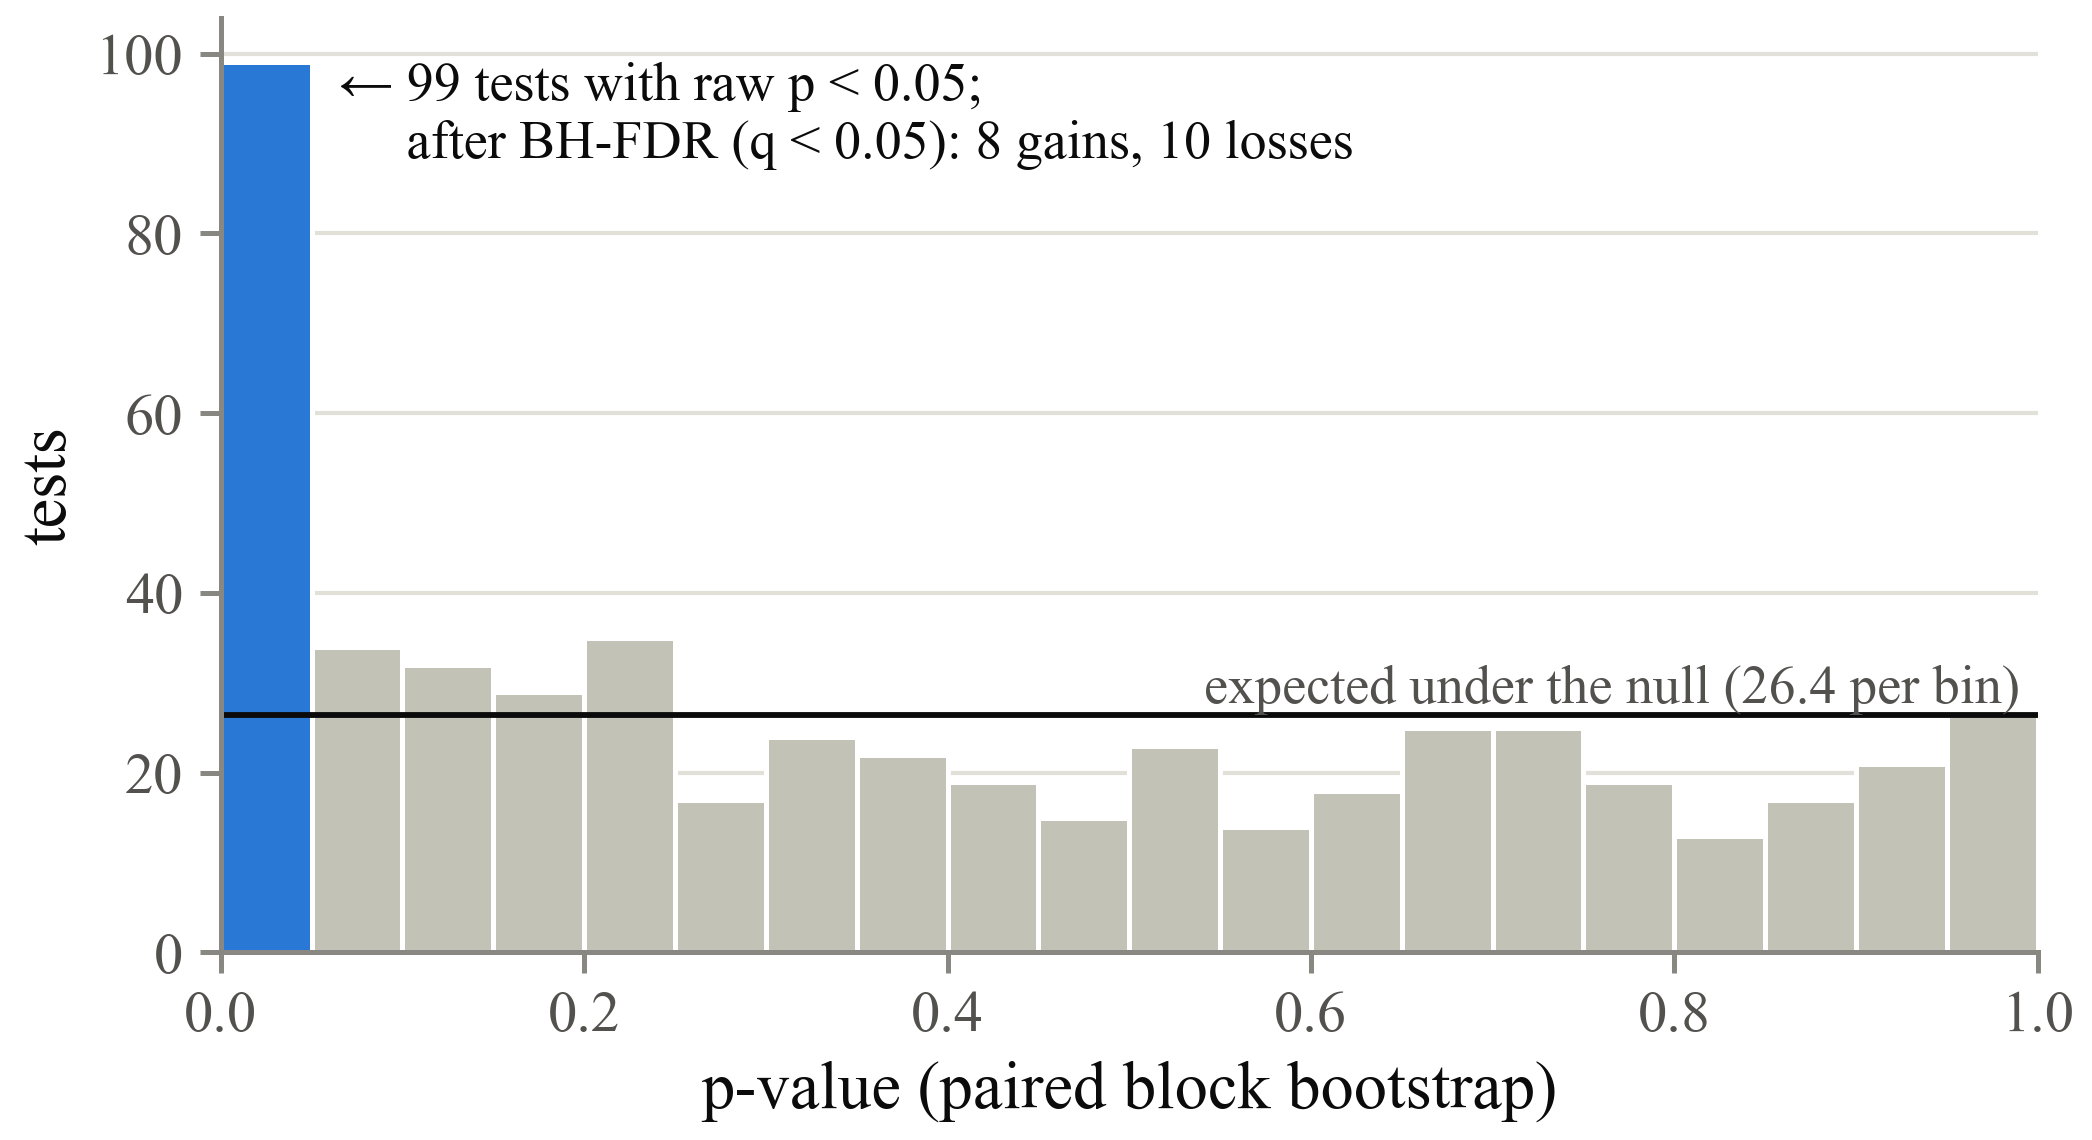
\includegraphics[width=3.487in]{figures/s2_pvalues.png}
\caption{Distribution of the \STwoMktTests{} market-level $p$-values. The excess in the first bin shows that the
components change performance; FDR control leaves few of those changes significant.}
\label{fig:pvalues}
\end{figure}

\subsection{Component Attribution}

Table~\ref{tab:s2comp} and Figs.~\ref{fig:distribution} and~\ref{fig:s2heatmap} give the per-component picture, and
Table~\ref{tab:s2bystrat} breaks it down by strategy. Four regularities refine the taxonomy of
Section~\ref{sec:taxonomy}.

\emph{Narrowing components are the most consistently positive and never significantly harmful.} Meta-labeling improves
the Sharpe ratio in \STwoMktMetaPos{} of market-level cells (median \STwoMktMetaMed{}; \STwoMktMetaGain{} significant
gain, \STwoMktMetaLoss{} significant losses), meta-label + sizing in \STwoMktBestPos{} (median \STwoMktBestMed{}), and
position sizing in \STwoMktSizingPos{} (median \STwoMktSizingMed{}, with no significant result in either direction).
Both also cut turnover, by a median of \STwoMktMetaTurn{} and \STwoMktBestTurn{} capital per year. Their gains are
small relative to their uncertainty.

\emph{ML entry is the most harmful component.} It loses in most cells (median \STwoMktEntryMed{};
\STwoMktEntryLoss{} significant losses) and raises turnover by \STwoMktEntryTurn{} capital per year. The damage is
concentrated in the contrarian strategy: \STwoMktEntryLossRSI{} of its significant losses are RSI(2) cells (median
\STwoMktEntryMedRSI{}), where a learned, trend-oriented entry replaces a mean-reversion rule.

\emph{ML exit is strategy dependent rather than uniformly harmful.} For the four trend-following controls its median
effect is \STwoMktExitMedTrend{}, but for RSI(2) it is \STwoMktExitMedRSI{}, with \STwoMktExitGainRSI{} significant
gains---the only component that significantly improves a strategy in several markets (all-market portfolio,
F\STwoFzA{}: \STwoGRSIExitADelta{}, CI \STwoGRSIExitACI{}). The RSI(2) rule's fixed ATR profit target caps winners, and
a learned continuation exit lets them run; for trend-followers, whose trailing stops already let winners run, the
learned exit mostly adds turnover (median \STwoMktExitTurn{}).

\emph{Independent gates do nothing reliable.} The ML regime filter (median \STwoMktRegimeMed{},
\STwoMktRegimeLoss{} significant results) and the rule-based ADX gate (median \STwoMktAdxMed{}, \STwoMktAdxLoss{}
significant loss) are indistinguishable from zero.

\begin{table*}[!t]
\centering
\caption{Component attribution across the universe. Market-level tests: every strategy $\times$ market $\times$ freeze. Sig.\ $+$/$-$ = BH-FDR $q<0.05$ within the family. Global = all-market portfolio (strategy $\times$ freeze). Freeze agreement = share of strategy $\times$ market cells whose $\Delta$SR has the same sign in both independent freezes. $\Delta$Turn.\ in capital/year.}
\label{tab:s2comp}
\footnotesize
\begin{tabular}{l l r r r r r r r r r}
\toprule
Component & Type & Tests & $\Delta$SR$>0$ & Median $\Delta$SR & Sig.$+$ & Sig.$-$ & Global median & Global $>0$ & Freeze agree & $\Delta$Turn. \\
\midrule
Rule ADX gate & rule & 80 & 46.2\% & -0.01 & 0 & 1 & -0.02 & 5/10 & 60.0\% & -2.36 \\
ML regime filter & independent & 75 & 45.3\% & -0.01 & 0 & 0 & -0.02 & 5/10 & 51.4\% & -3.39 \\
ML meta-labeling & narrowing & 74 & 67.6\% & +0.12 & 1 & 0 & +0.08 & 6/10 & 74.3\% & -4.42 \\
ML position sizing & narrowing & 75 & 70.7\% & +0.05 & 0 & 0 & +0.03 & 6/10 & 54.3\% & -1.67 \\
ML entry & replacing & 75 & 40.0\% & -0.15 & 0 & 8 & -0.24 & 2/10 & 74.3\% & +9.54 \\
ML exit & replacing & 75 & 48.0\% & -0.03 & 6 & 1 & -0.17 & 3/10 & 74.3\% & +4.87 \\
Meta-label + sizing & combination & 74 & 67.6\% & +0.12 & 1 & 0 & +0.08 & 6/10 & 74.3\% & -2.79 \\
\bottomrule
\end{tabular}
\end{table*}


\begin{figure}[!t]
\centering
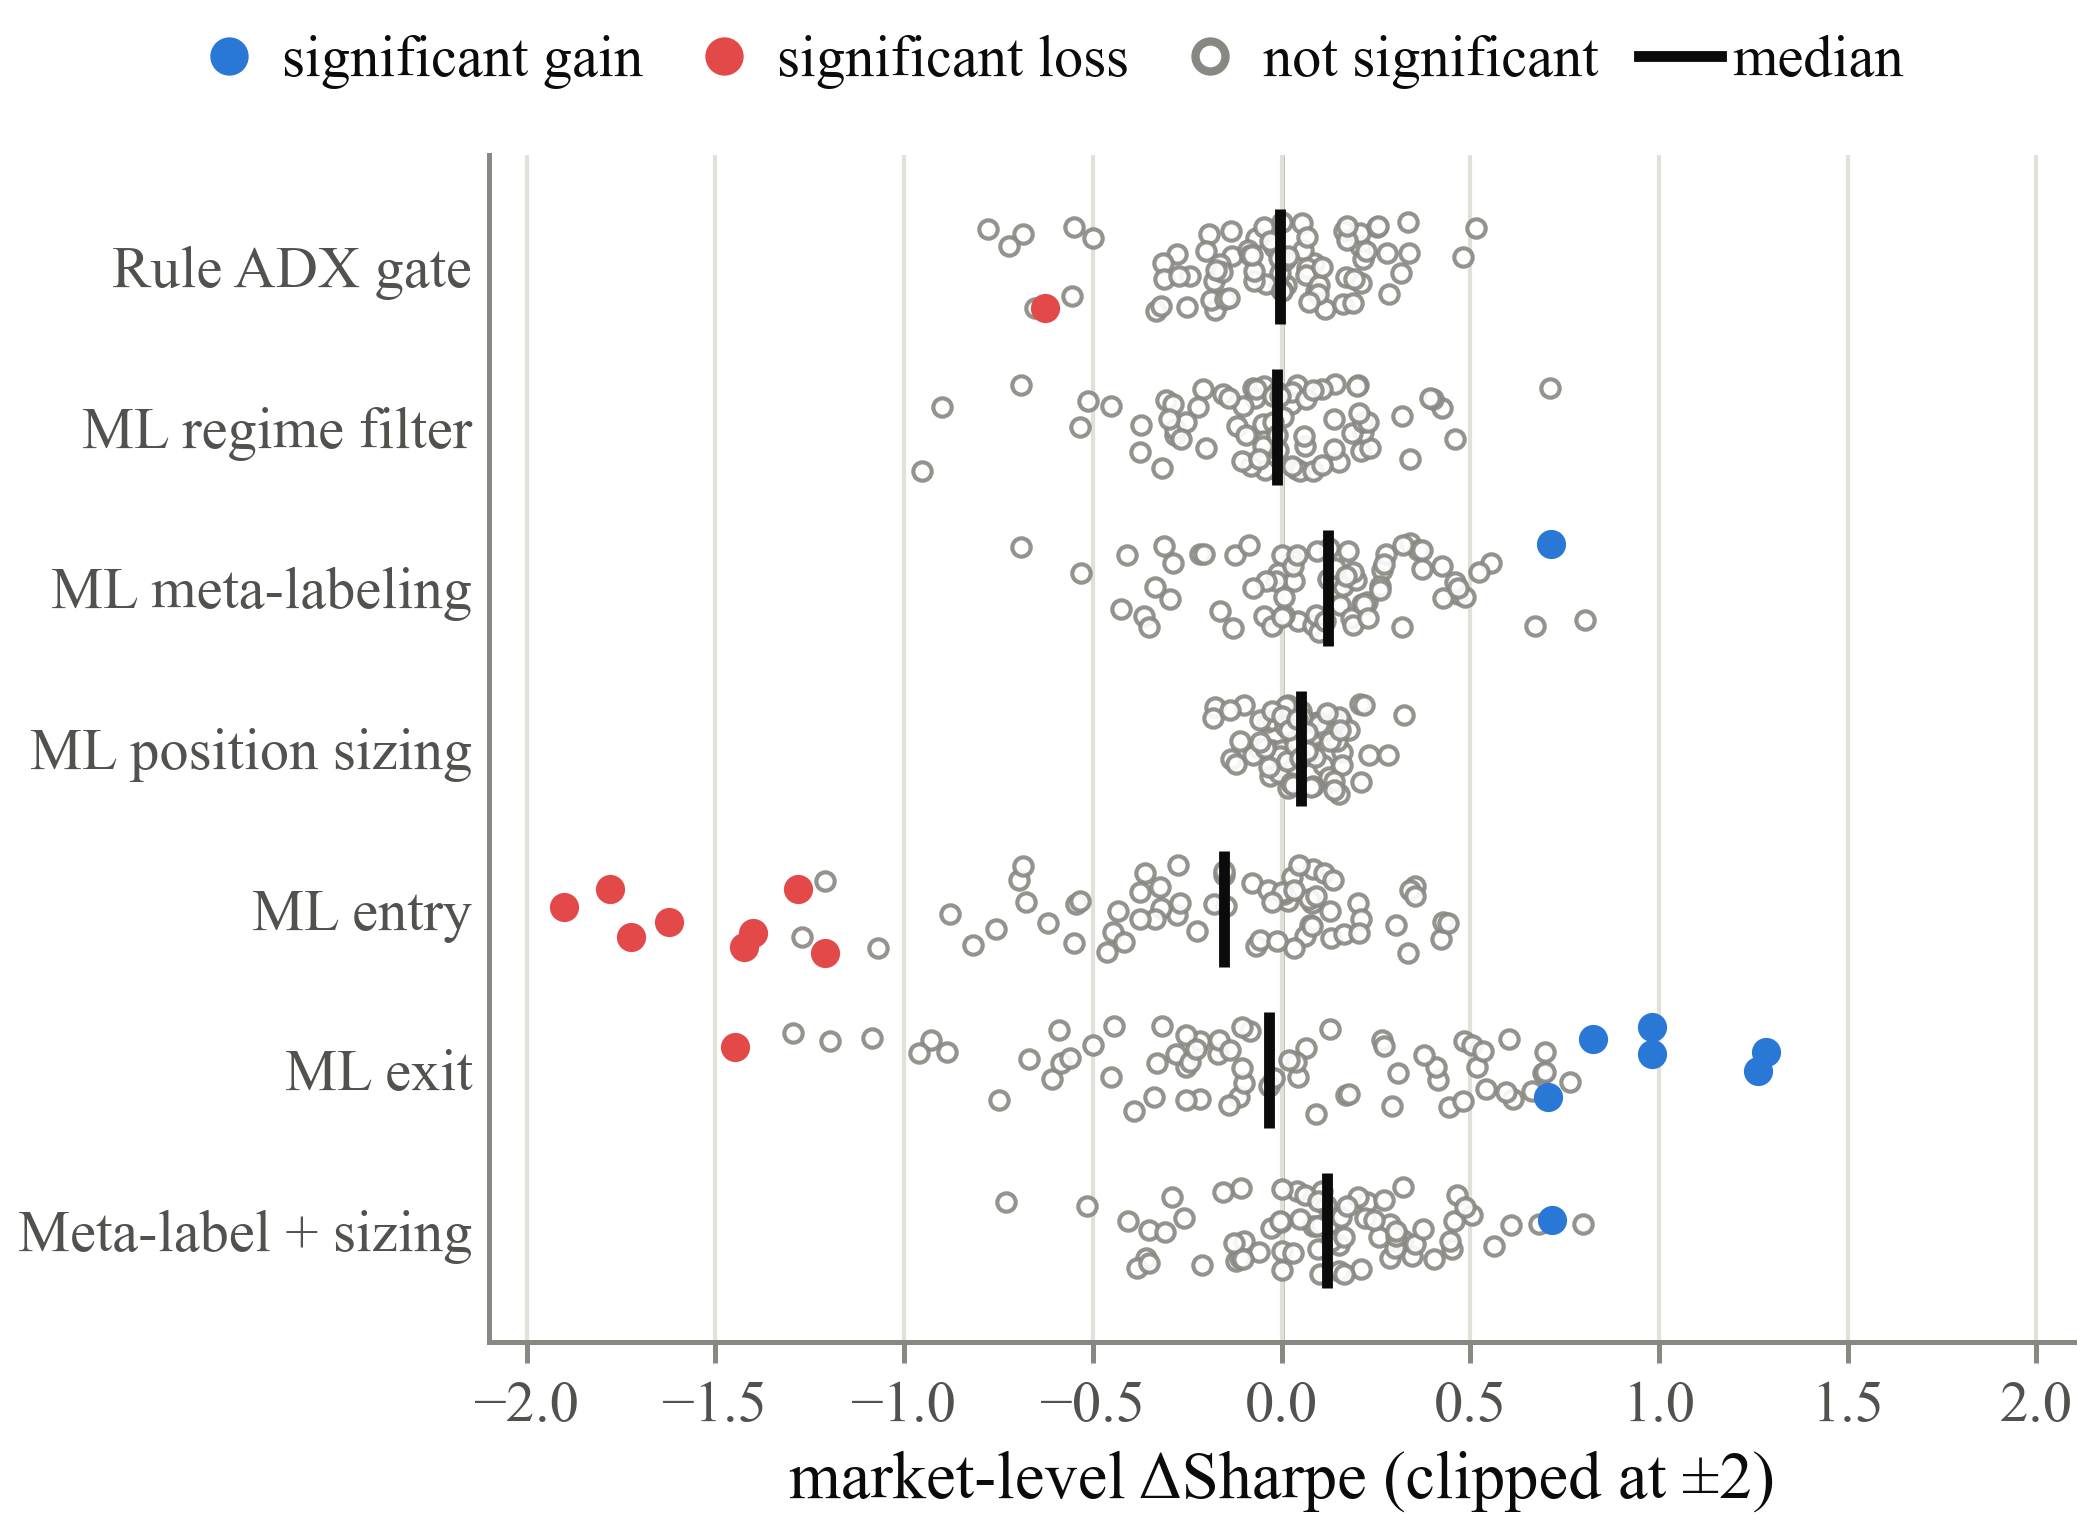
\includegraphics[width=3.487in]{figures/s2_distribution.png}
\caption{Every market-level $\Delta$Sharpe, by component. Filled markers are significant at $q < \STwoAlpha$;
vertical bars mark the median.}
\label{fig:distribution}
\end{figure}

\begin{figure*}[!t]
\centering
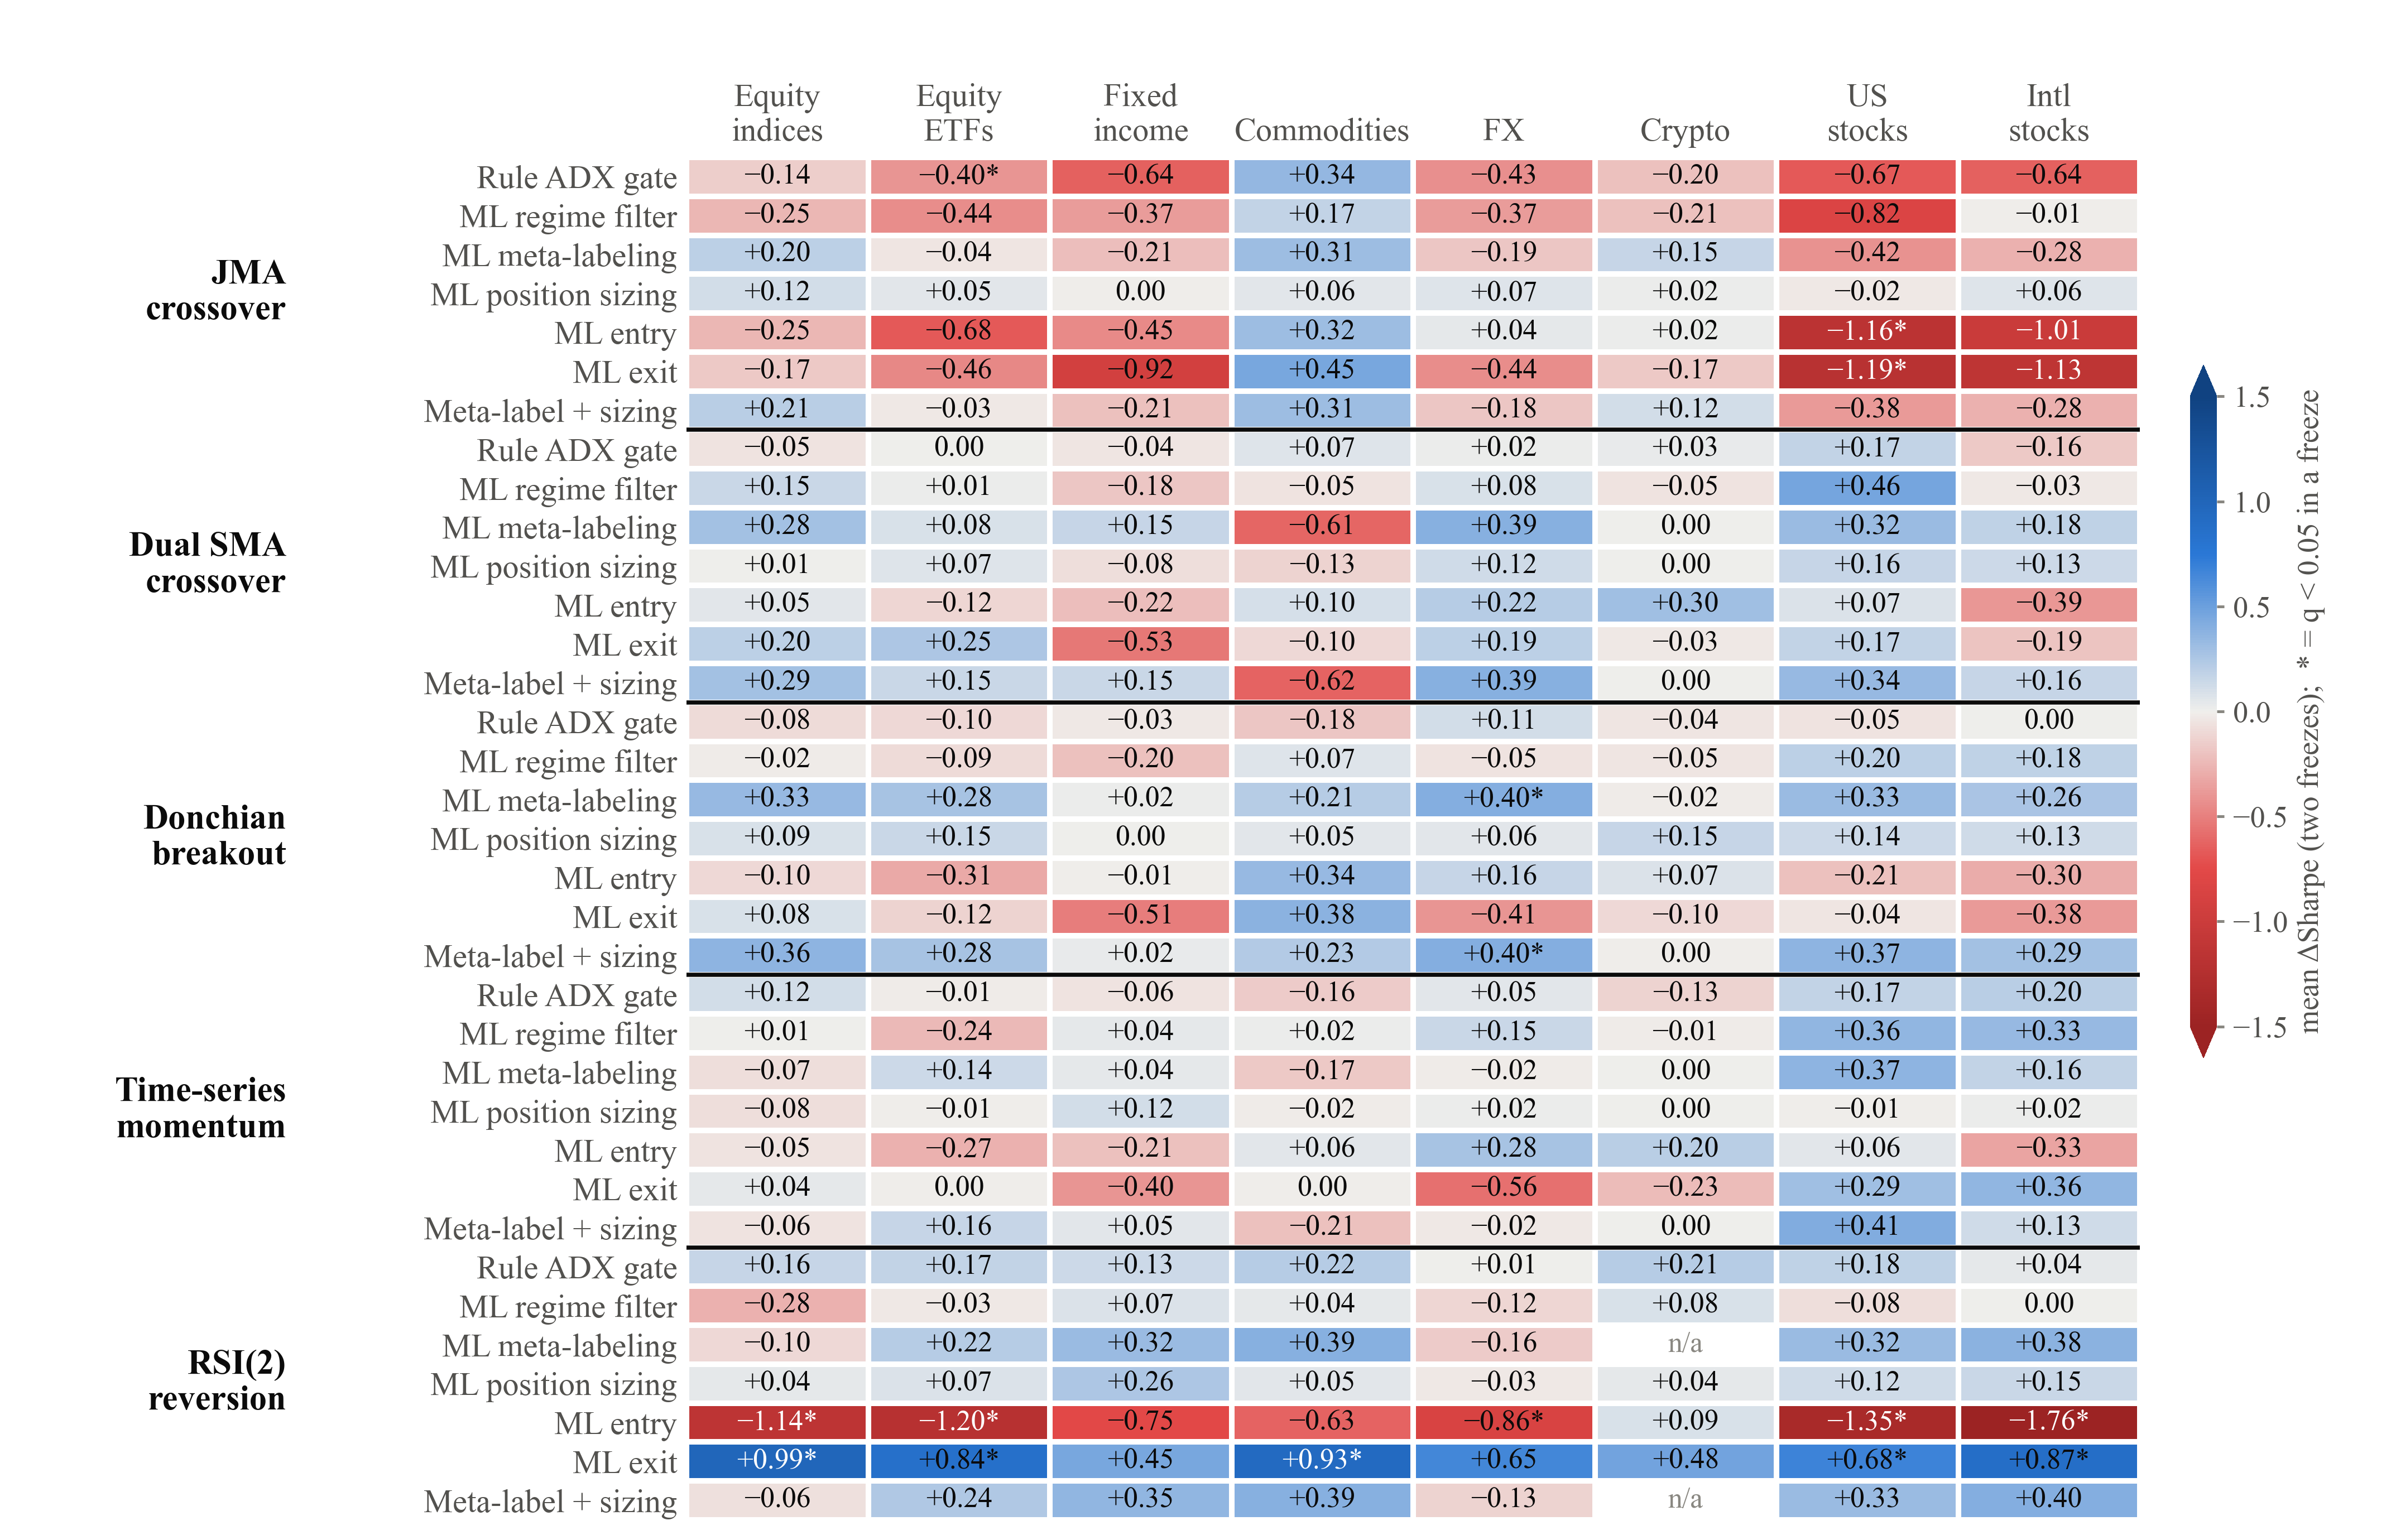
\includegraphics[width=7.14in]{figures/s2_heatmap.png}
\caption{Where ML changes each strategy: mean $\Delta$Sharpe over the two freezes for every strategy, component, and
market (* = significant at $q < \STwoAlpha$ in at least one freeze; n/a = no training data). The ML exit and ML entry
rows of RSI(2) reversion carry most of the significant cells.}
\label{fig:s2heatmap}
\end{figure*}

\begin{longtable}{p{2.4cm} r r r r r r r }
\caption{Median market-level $\Delta$SR by strategy and component (significant gains / significant losses at $q<0.05$ in parentheses).} \label{tab:s2bystrat} \\
\toprule
Strategy & Rule ADX gate & ML regime filter & ML meta-labeling & ML position sizing & ML entry & ML exit & Meta-label + sizing \\
\midrule
\endhead
\bottomrule
\endfoot
JMA crossover & -0.42 (0/1) & -0.28 (0/0) & -0.12 (0/0) & +0.05 (0/0) & -0.28 (0/1) & -0.59 (0/1) & -0.11 (0/0) \\
Dual SMA crossover & +0.01 (0/0) & -0.01 (0/0) & +0.21 (0/0) & +0.04 (0/0) & +0.06 (0/0) & -0.08 (0/0) & +0.21 (0/0) \\
Donchian breakout & -0.04 (0/0) & +0.00 (0/0) & +0.18 (1/0) & +0.10 (0/0) & -0.06 (0/0) & -0.14 (0/0) & +0.22 (1/0) \\
Time-series momentum & +0.03 (0/0) & +0.06 (0/0) & +0.09 (0/0) & +0.00 (0/0) & +0.00 (0/0) & -0.11 (0/0) & +0.10 (0/0) \\
RSI(2) reversion & +0.14 (0/0) & -0.06 (0/0) & +0.20 (0/0) & +0.08 (0/0) & -1.07 (0/7) & +0.70 (6/0) & +0.21 (0/0) \\
\end{longtable}


\subsection{The All-Market Portfolio}

Fig.~\ref{fig:s2forest} reports every global before-and-after comparison with its paired bootstrap CI,
Fig.~\ref{fig:s2equity} the corresponding equity curves, and Fig.~\ref{fig:s2risk} the change in the full risk
profile. Two facts frame all ML effects. First, the rule-based controls are weak out of sample: their all-market
Sharpe ratios range from \STwoGRSIBaseA{} (RSI(2), F\STwoFzA{}) to \STwoGJMABaseA{} (JMA, F\STwoFzA{}). Second, most
drawdown changes are mechanical exposure effects rather than skill. Every component that trades less makes the
all-market maximum drawdown shallower in most cases (meta-labeling \STwoGlobMetaDD{}, meta-label + sizing
\STwoGlobBestDD{}, ML exit \STwoGlobExitDD{}, ML regime filter \STwoGlobRegimeDD{}; median exposure change
\STwoGlobMetaExp{}, \STwoGlobBestExp{}, \STwoGlobExitExp{}, and \STwoGlobRegimeExp{}), whereas ML entry, which raises
exposure by \STwoGlobEntryExp{}, deepens it in every case (\STwoGlobEntryDD{} shallower). The risk-adjusted return,
not the drawdown, is therefore the right yardstick for attribution.

\begin{figure*}[!t]
\centering
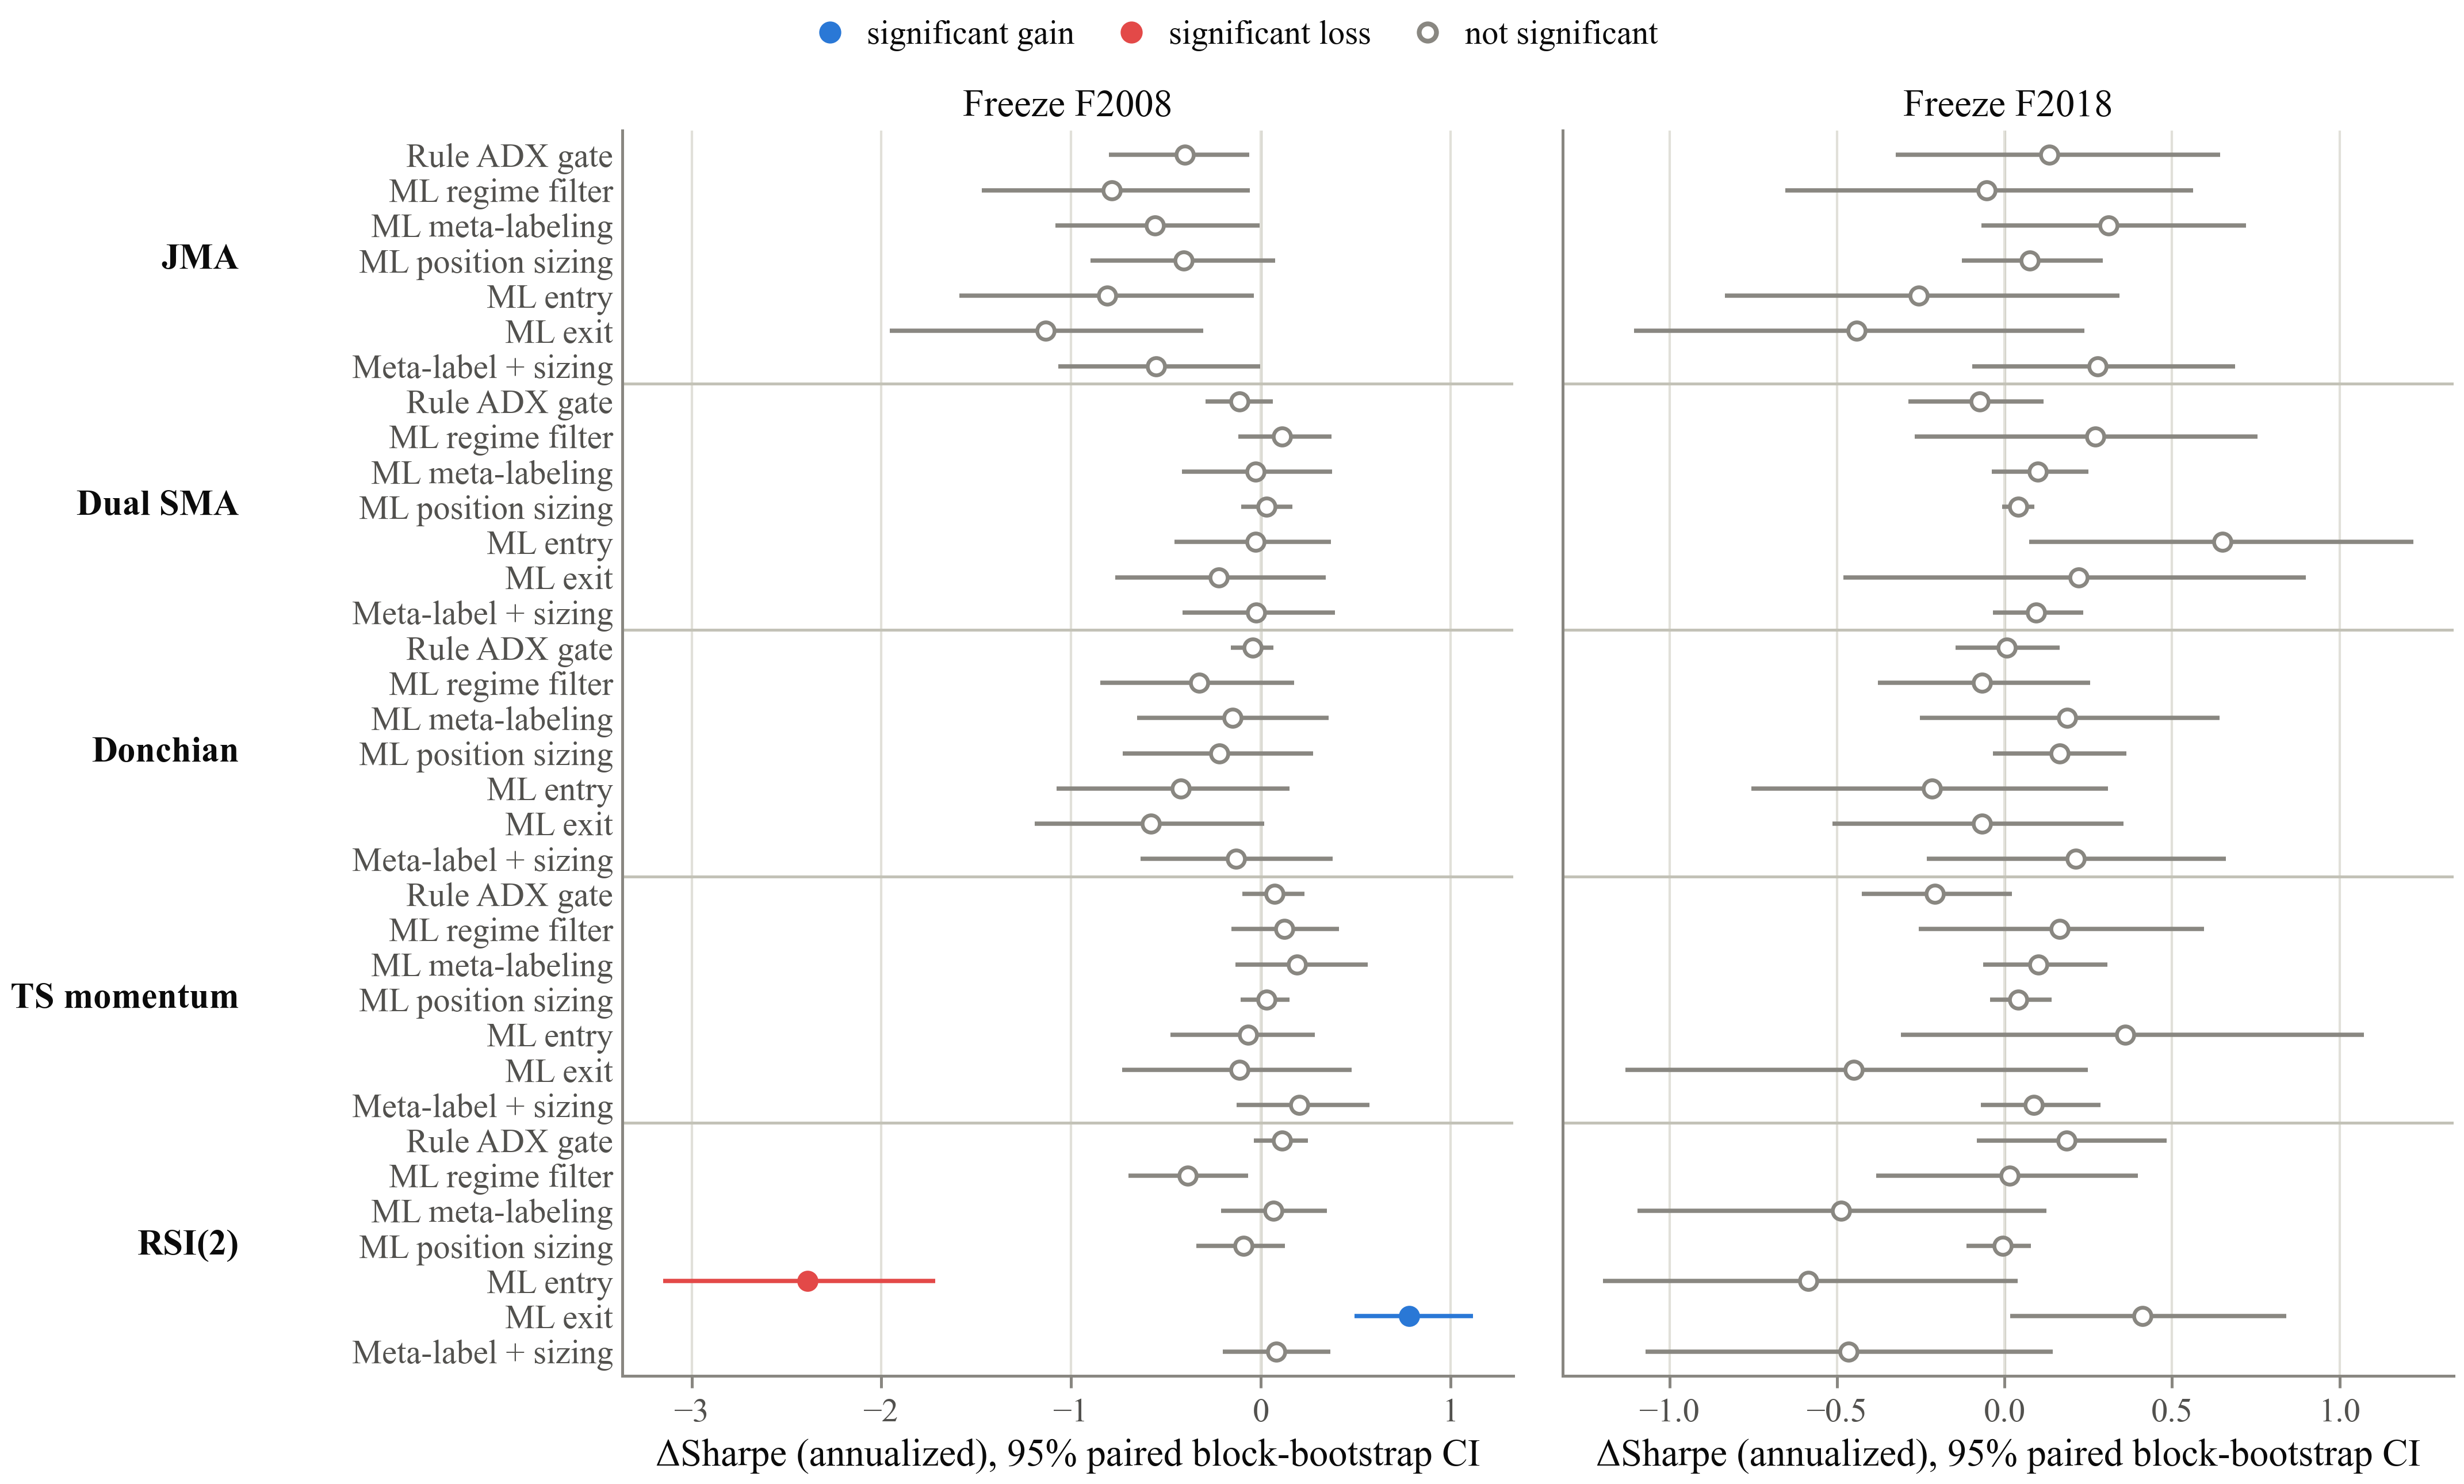
\includegraphics[width=7.14in]{figures/s2_forest_global.png}
\caption{All-market portfolio: $\Delta$Sharpe with 95\% paired block-bootstrap CIs for every strategy and component,
in each freeze. Filled markers are significant at $q < \STwoAlpha$ across the \STwoGlobTests{} global tests.}
\label{fig:s2forest}
\end{figure*}

\begin{figure*}[!t]
\centering
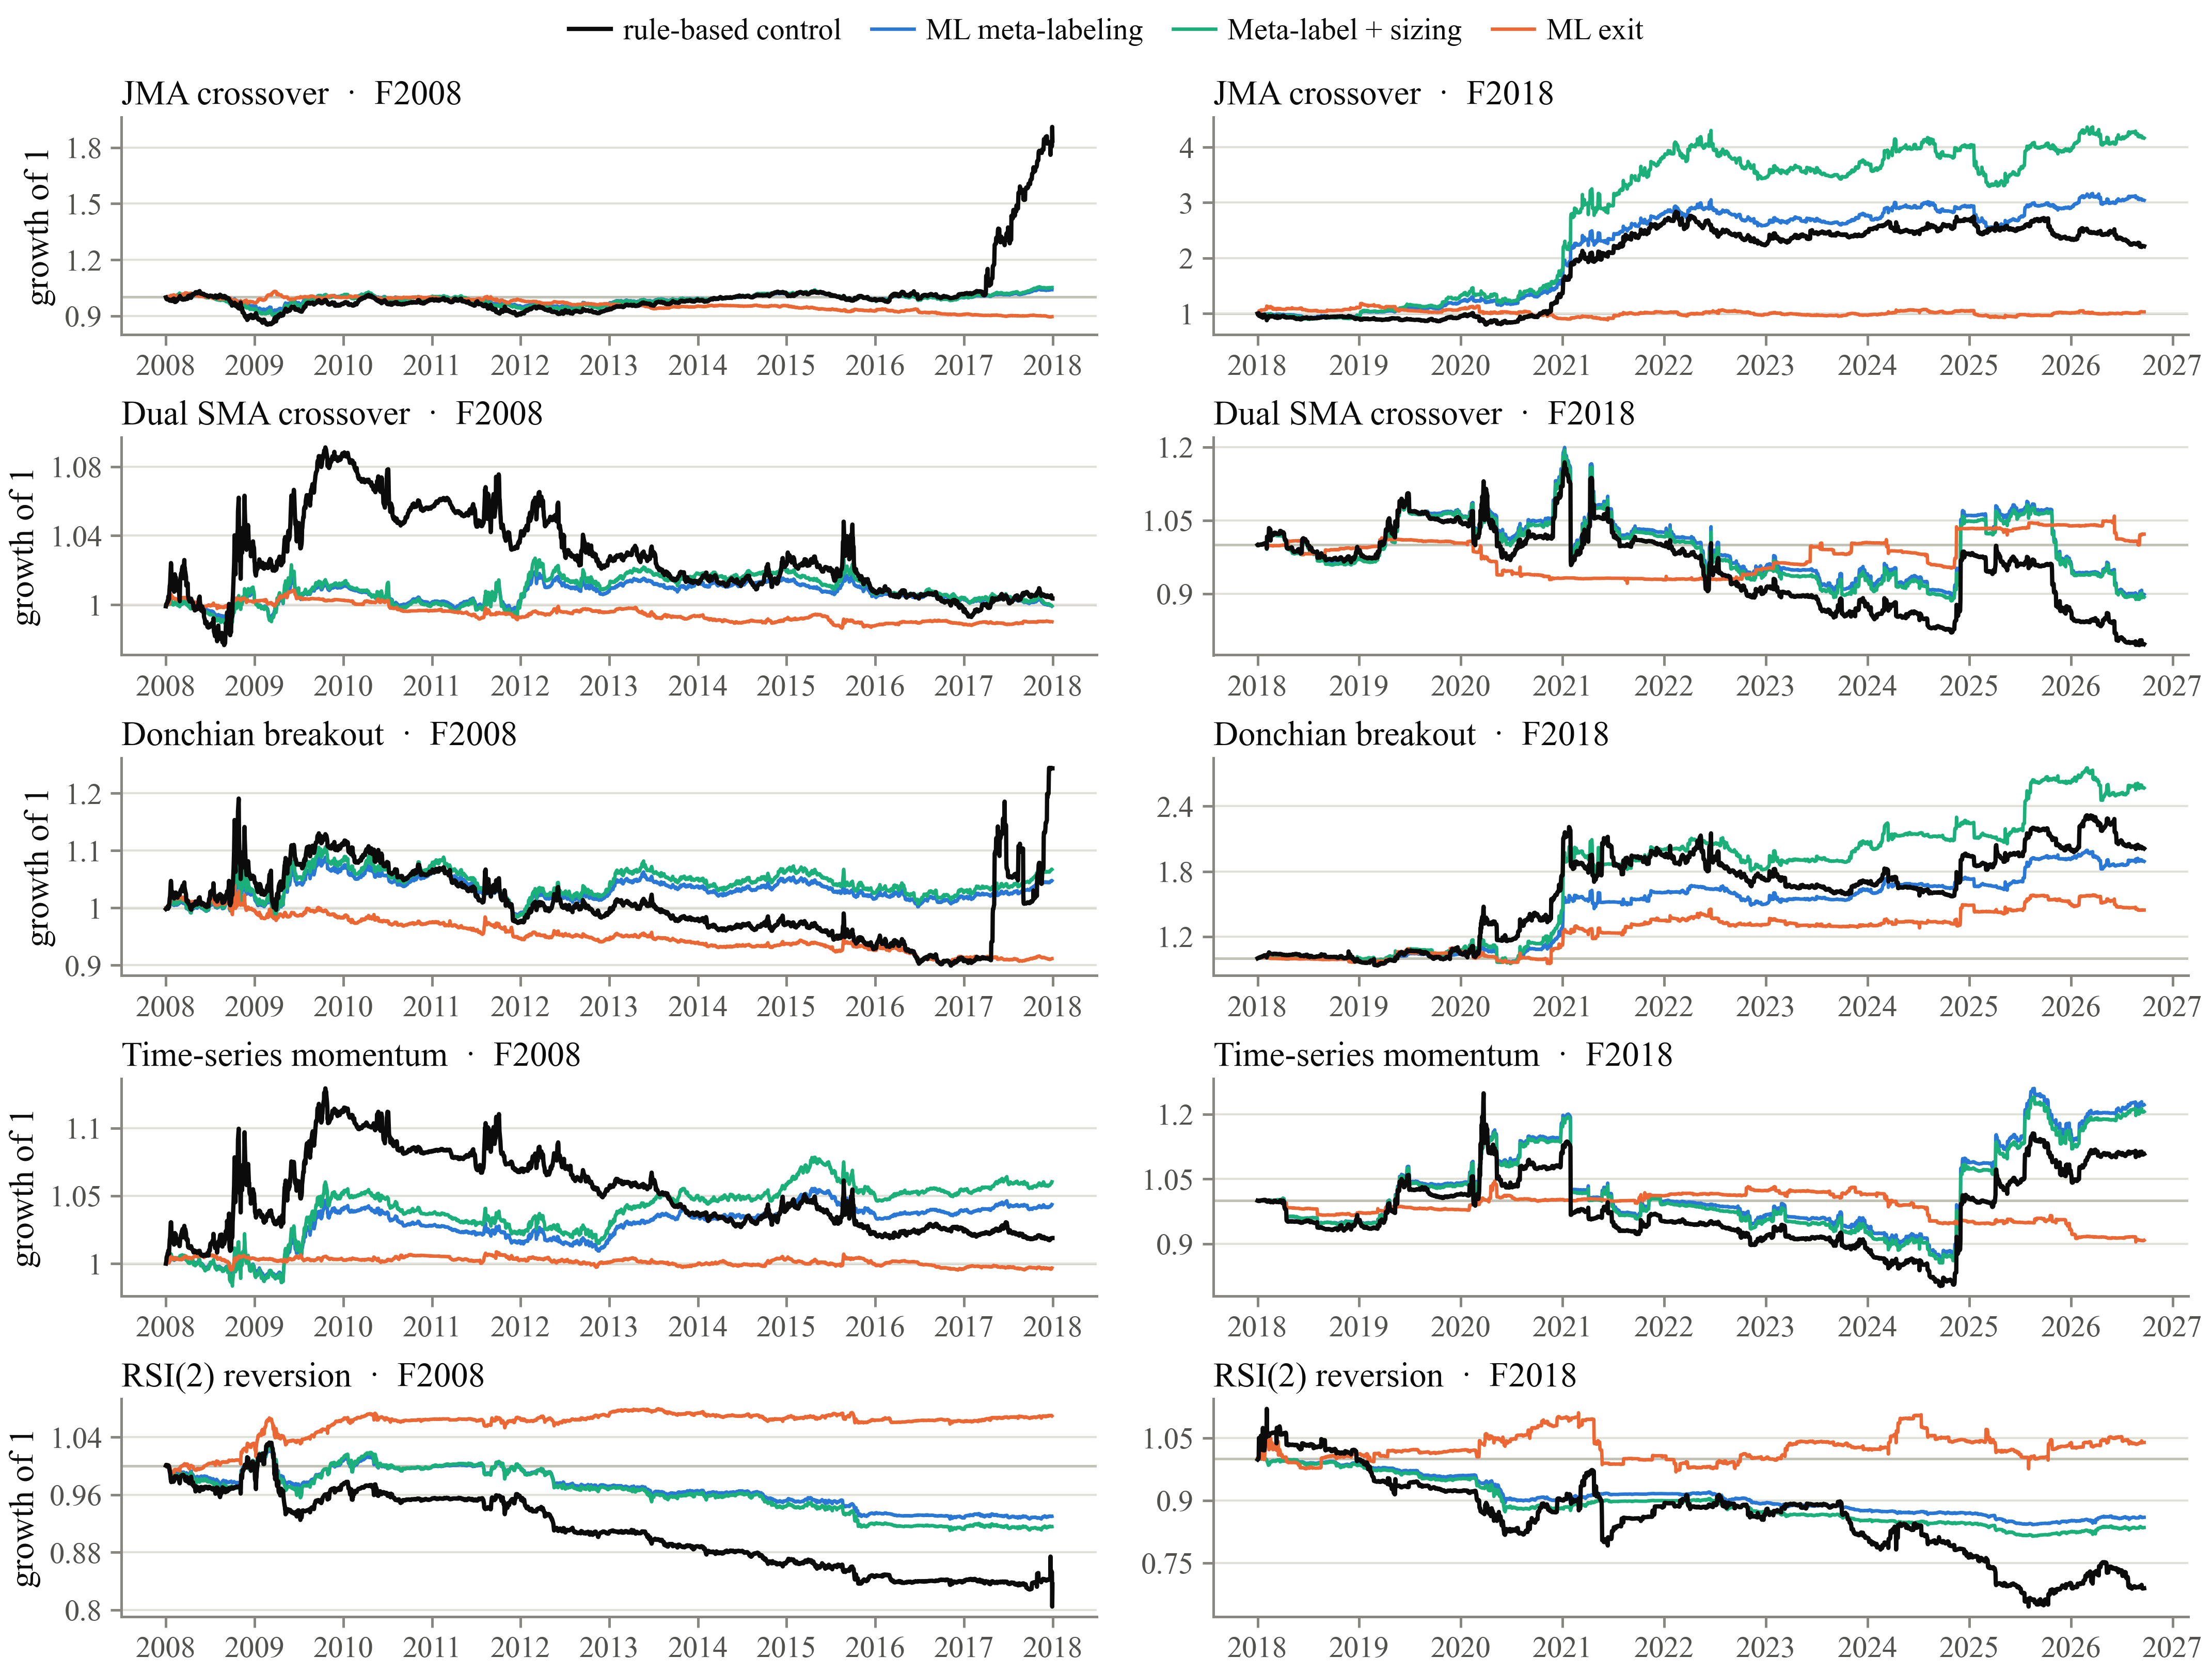
\includegraphics[width=7.14in]{figures/s2_equity.png}
\caption{All-market equity curves (growth of one unit of capital) in each out-of-sample window: the rule-based
control against meta-labeling, meta-label + sizing, and ML exit.}
\label{fig:s2equity}
\end{figure*}

\begin{figure*}[!t]
\centering
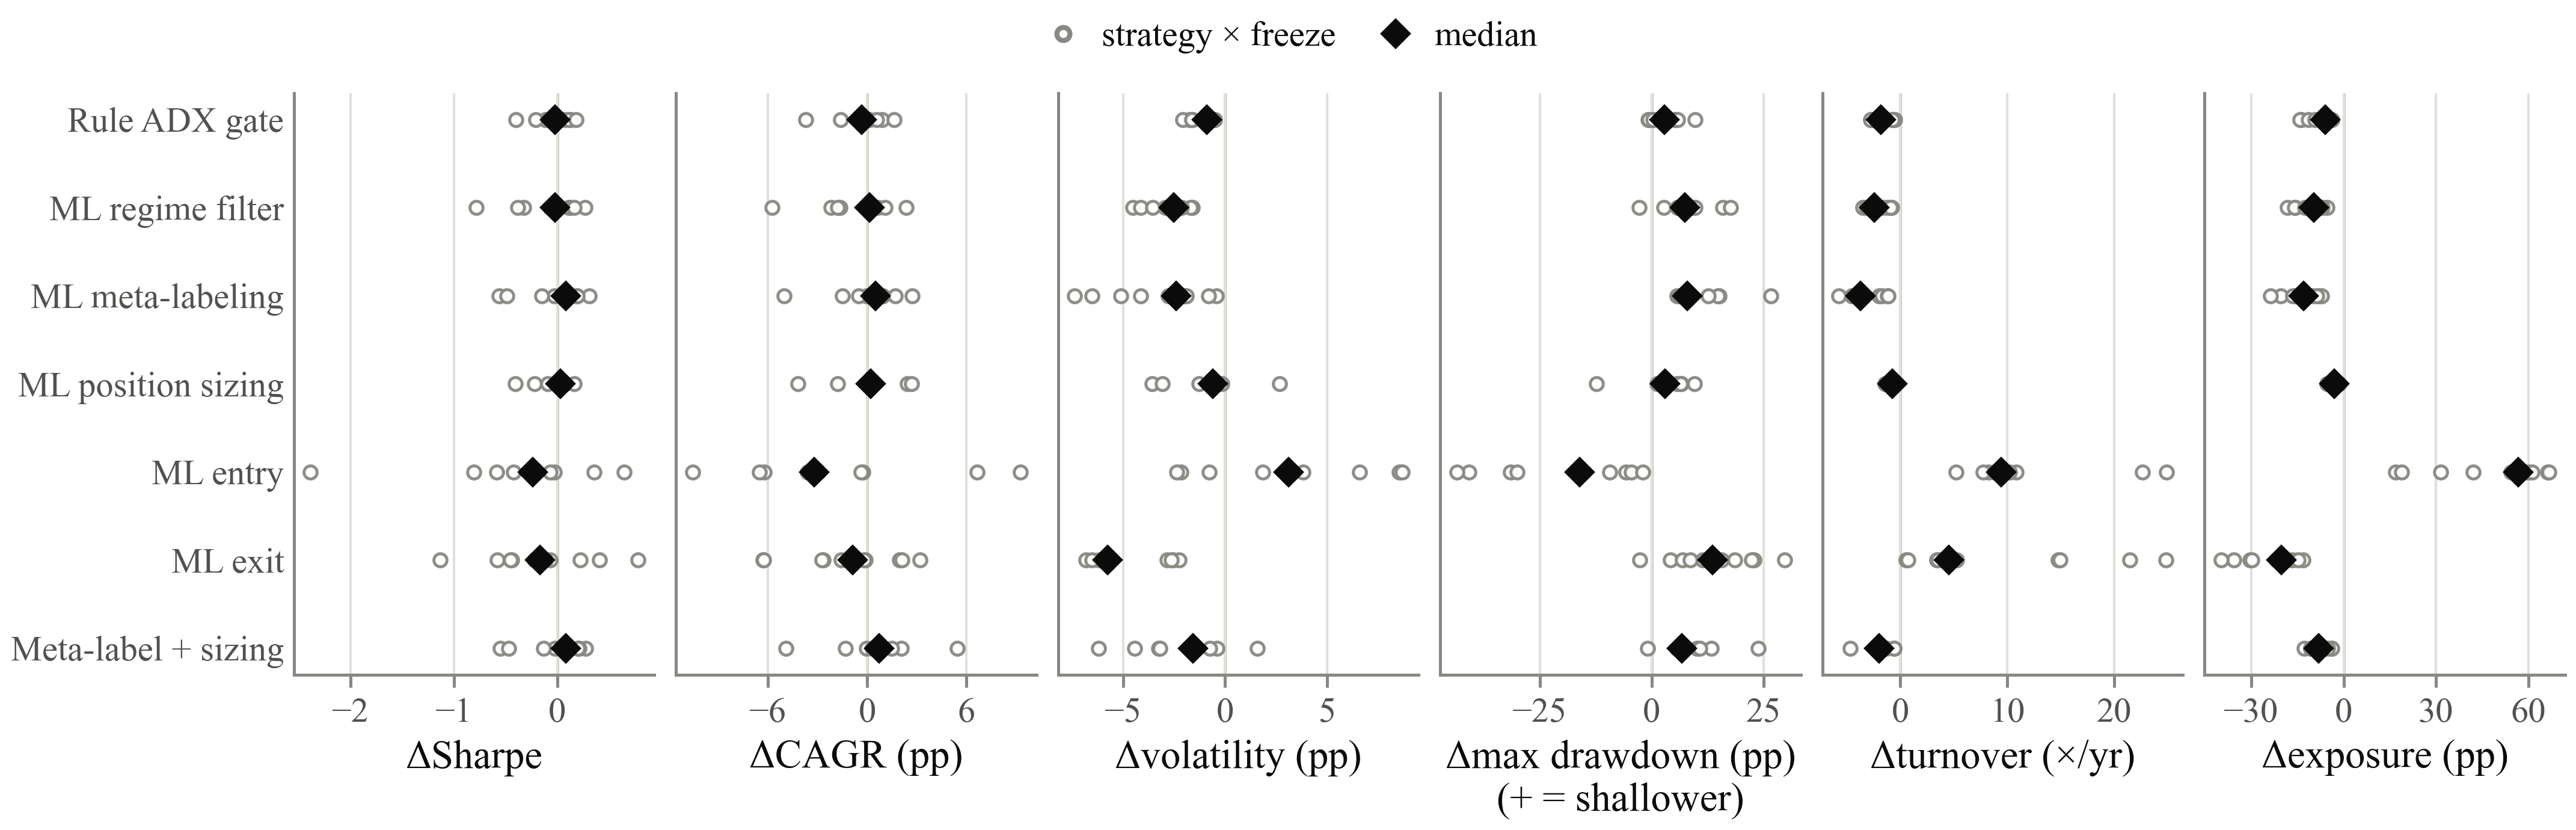
\includegraphics[width=7.14in]{figures/s2_risk.png}
\caption{Change in the all-market risk profile, variant minus control, for each strategy $\times$ freeze cell (open
circles) and its median (diamond). Drawdown changes track exposure changes: components that trade less have
shallower drawdowns.}
\label{fig:s2risk}
\end{figure*}

\subsection{Replication Across Freezes}

The two freezes are independent replications with different training data and non-overlapping test periods
(Fig.~\ref{fig:freezerep}); only cells observed in both freezes are compared. Agreement is modest. The sign of a
strategy $\times$ market effect agrees across freezes in \STwoRepMetaAgree{} of cells for meta-labeling,
\STwoRepBestAgree{} for meta-label + sizing, \STwoRepExitAgree{} for ML exit, and \STwoRepEntryAgree{} for ML entry,
but only \STwoRepRegimeAgree{} and \STwoRepSizingAgree{}---close to chance---for the regime filter and position
sizing. Magnitudes separate the components more clearly: the cross-freeze correlation of $\Delta$Sharpe is
\STwoRepExitCorr{} for exit and \STwoRepEntryCorr{} for entry, but \STwoRepMetaCorr{} for meta-labeling and
\STwoRepSizingCorr{} for sizing. The components with large effects replicate best; the small positive effects of the
narrowing components replicate in sign more often than in size.

\begin{figure*}[!t]
\centering
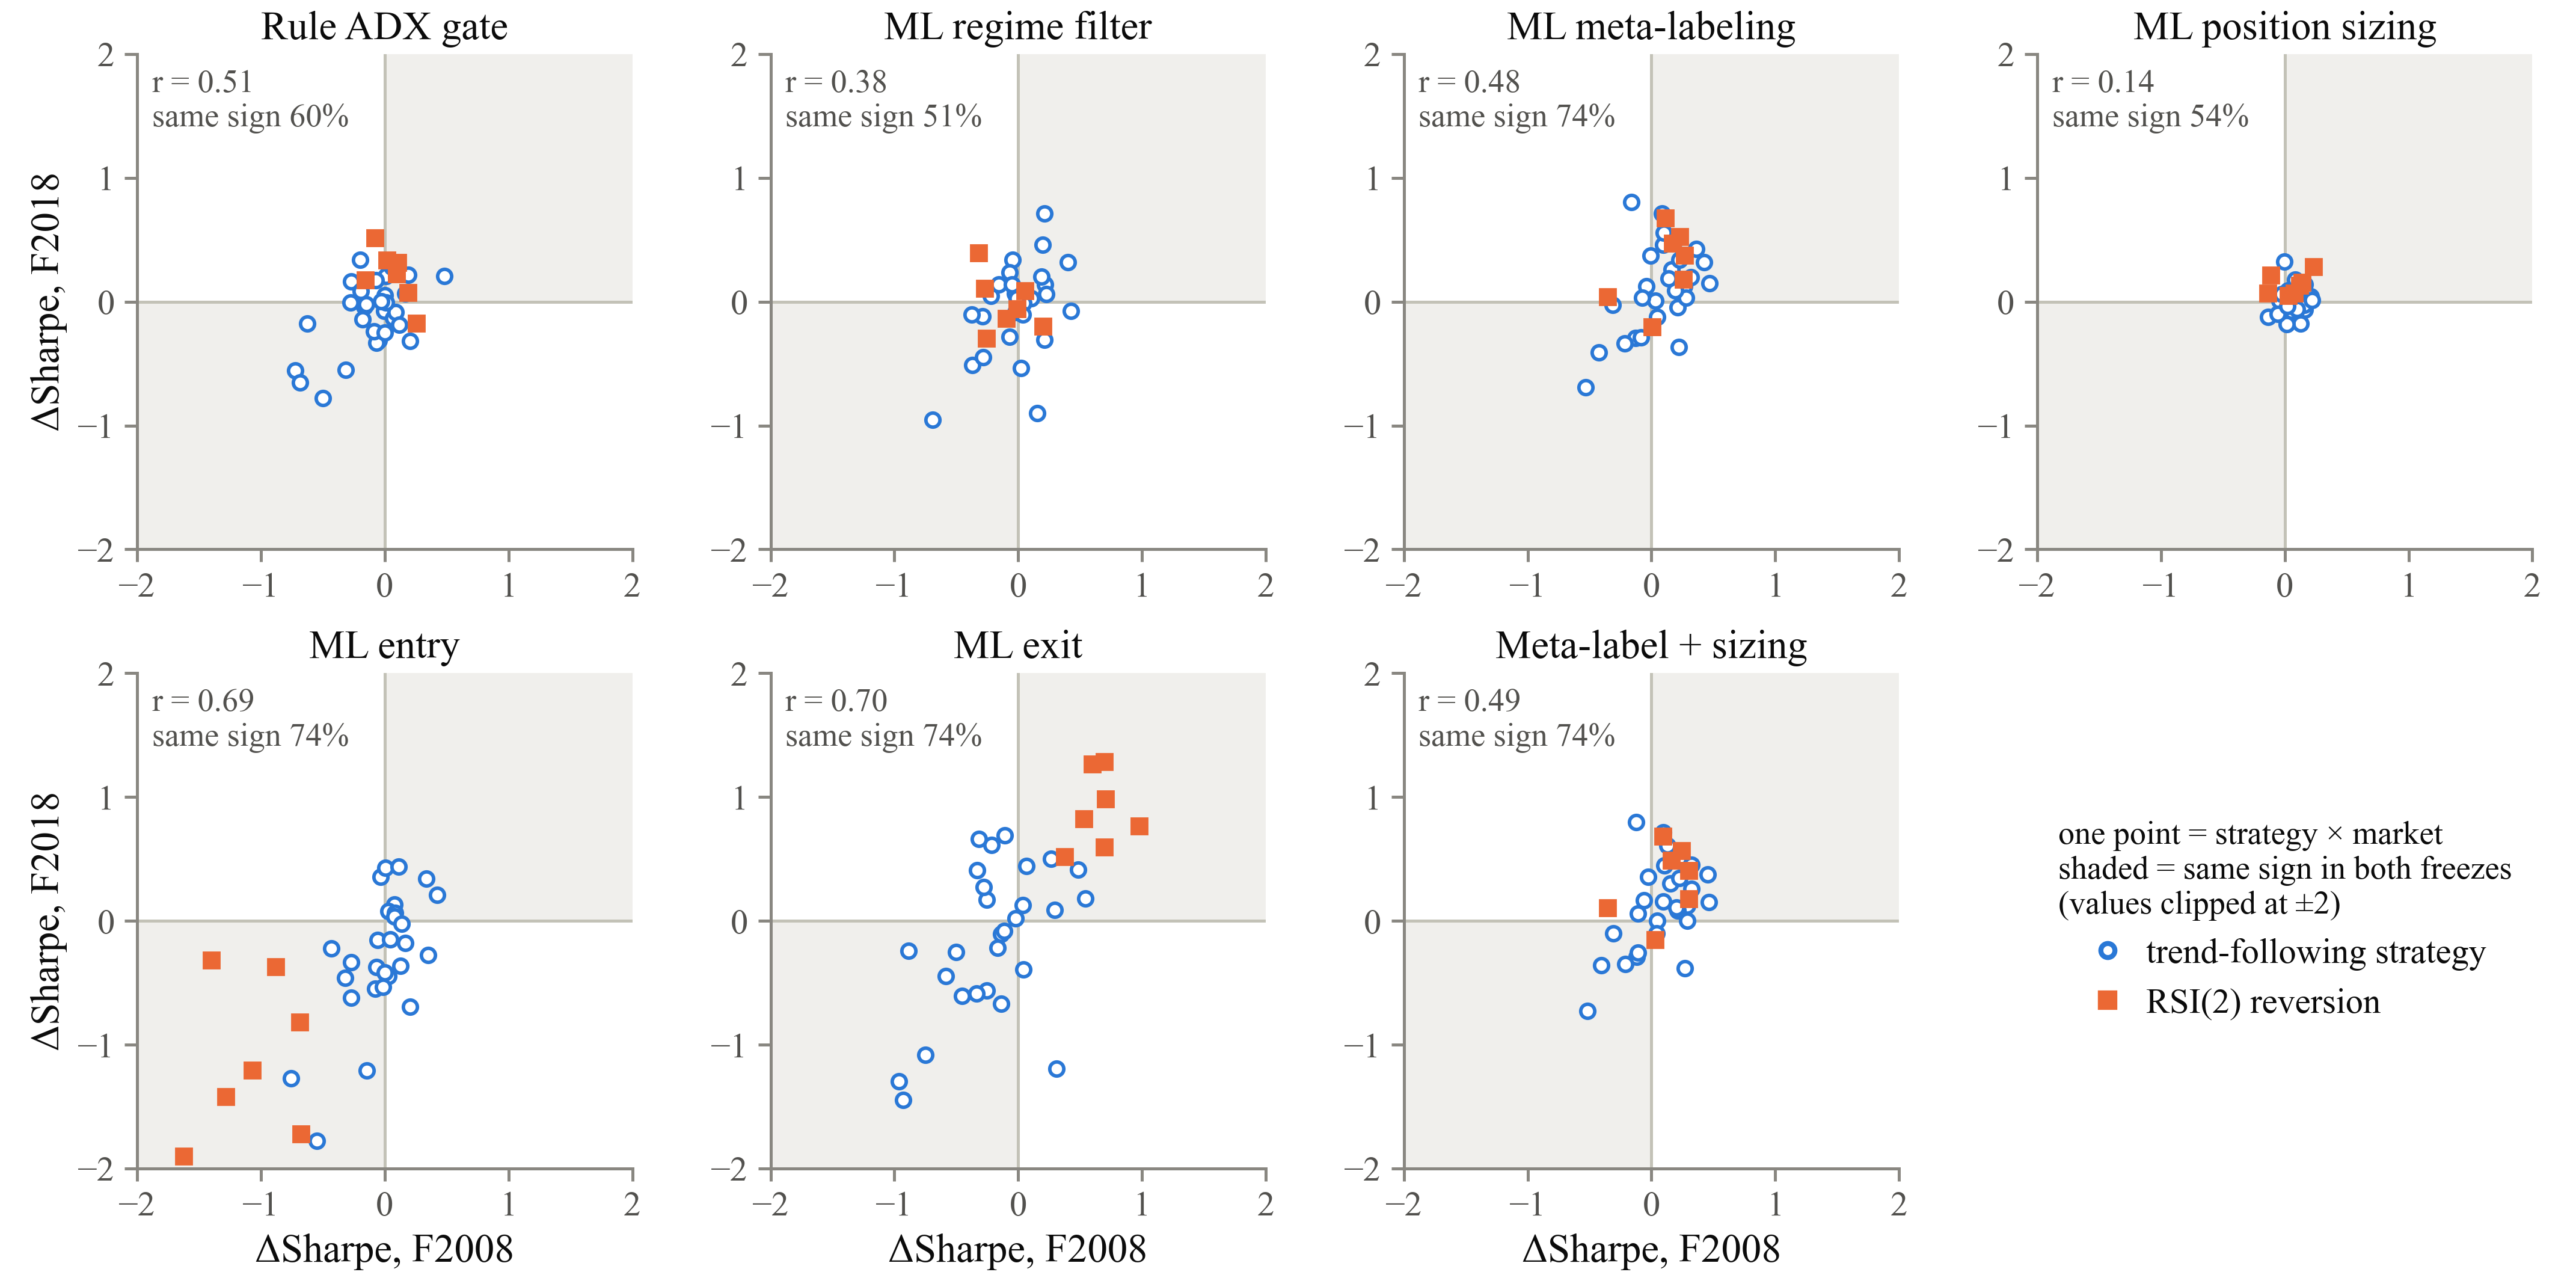
\includegraphics[width=7.14in]{figures/s2_freeze_rep.png}
\caption{Replication at a second freeze: market-level $\Delta$Sharpe in F\STwoFzA{} against F\STwoFzB{} for each
strategy $\times$ market cell, by component, with the cross-freeze correlation $r$ and sign-agreement rate.}
\label{fig:freezerep}
\end{figure*}

\subsection{Transfer, Budget, and Execution}

Fig.~\ref{fig:s2robust} collects three pre-registered robustness checks. \emph{Cross-market transfer} (panel a):
models fit on every other market and applied to a held-out one do at least as well as models fit in-market.
Transferred meta-labeling has a median $\Delta$Sharpe of \STwoTransferMetaMed{} (positive in \STwoTransferMetaPos{} of
cells, \STwoTransferMetaLoss{} significant losses) and transferred meta-label + sizing \STwoTransferBestMed{}
(\STwoTransferBestPos{}), against \STwoMktMetaMed{} and \STwoMktBestMed{} in-market, so whatever the meta-label model
learns is not market specific. \emph{Budget ablations} (panel b): moving the meta-label threshold to \STwoThrLo{} or
\STwoThrHi{} (median \STwoAblThrMed{} and \STwoAblThrHiMed{}) or shrinking the model to \STwoSmallTrees{} trees of
depth \STwoSmallDepth{} (meta-labeling \STwoAblMetaSmallMed{}, exit \STwoAblExitSmallMed{}) leaves the conclusions
unchanged; the effects come from the insertion point, not from the particular budget.

\emph{Execution assumptions} (panel c) matter more than any ML component. Filling a breached stop at the stop level
instead of at the breaching close---the Study~1 convention---raises the rule-based control's all-market Sharpe ratio
by \STwoExecBaseStopMin{} to \STwoExecBaseStopMax{} (significant in \STwoExecBaseStopSig{} strategy $\times$ freeze
cells). Under that optimistic fill, ML exit looks far worse (median \STwoExecExitStopMed{}, \STwoExecExitStopSig{}
significant) than under realistic fills (median \STwoGlobExitMed{}), because the fill flatters the control, not the
exit. Part of Study~1's finding that ML exit is harmful is therefore an artifact of optimistic stop fills. A one-day
entry lag changes the control by a median of \STwoExecBaseLagMed{} and leaves the ML comparisons qualitatively
unchanged.

\begin{figure*}[!t]
\centering
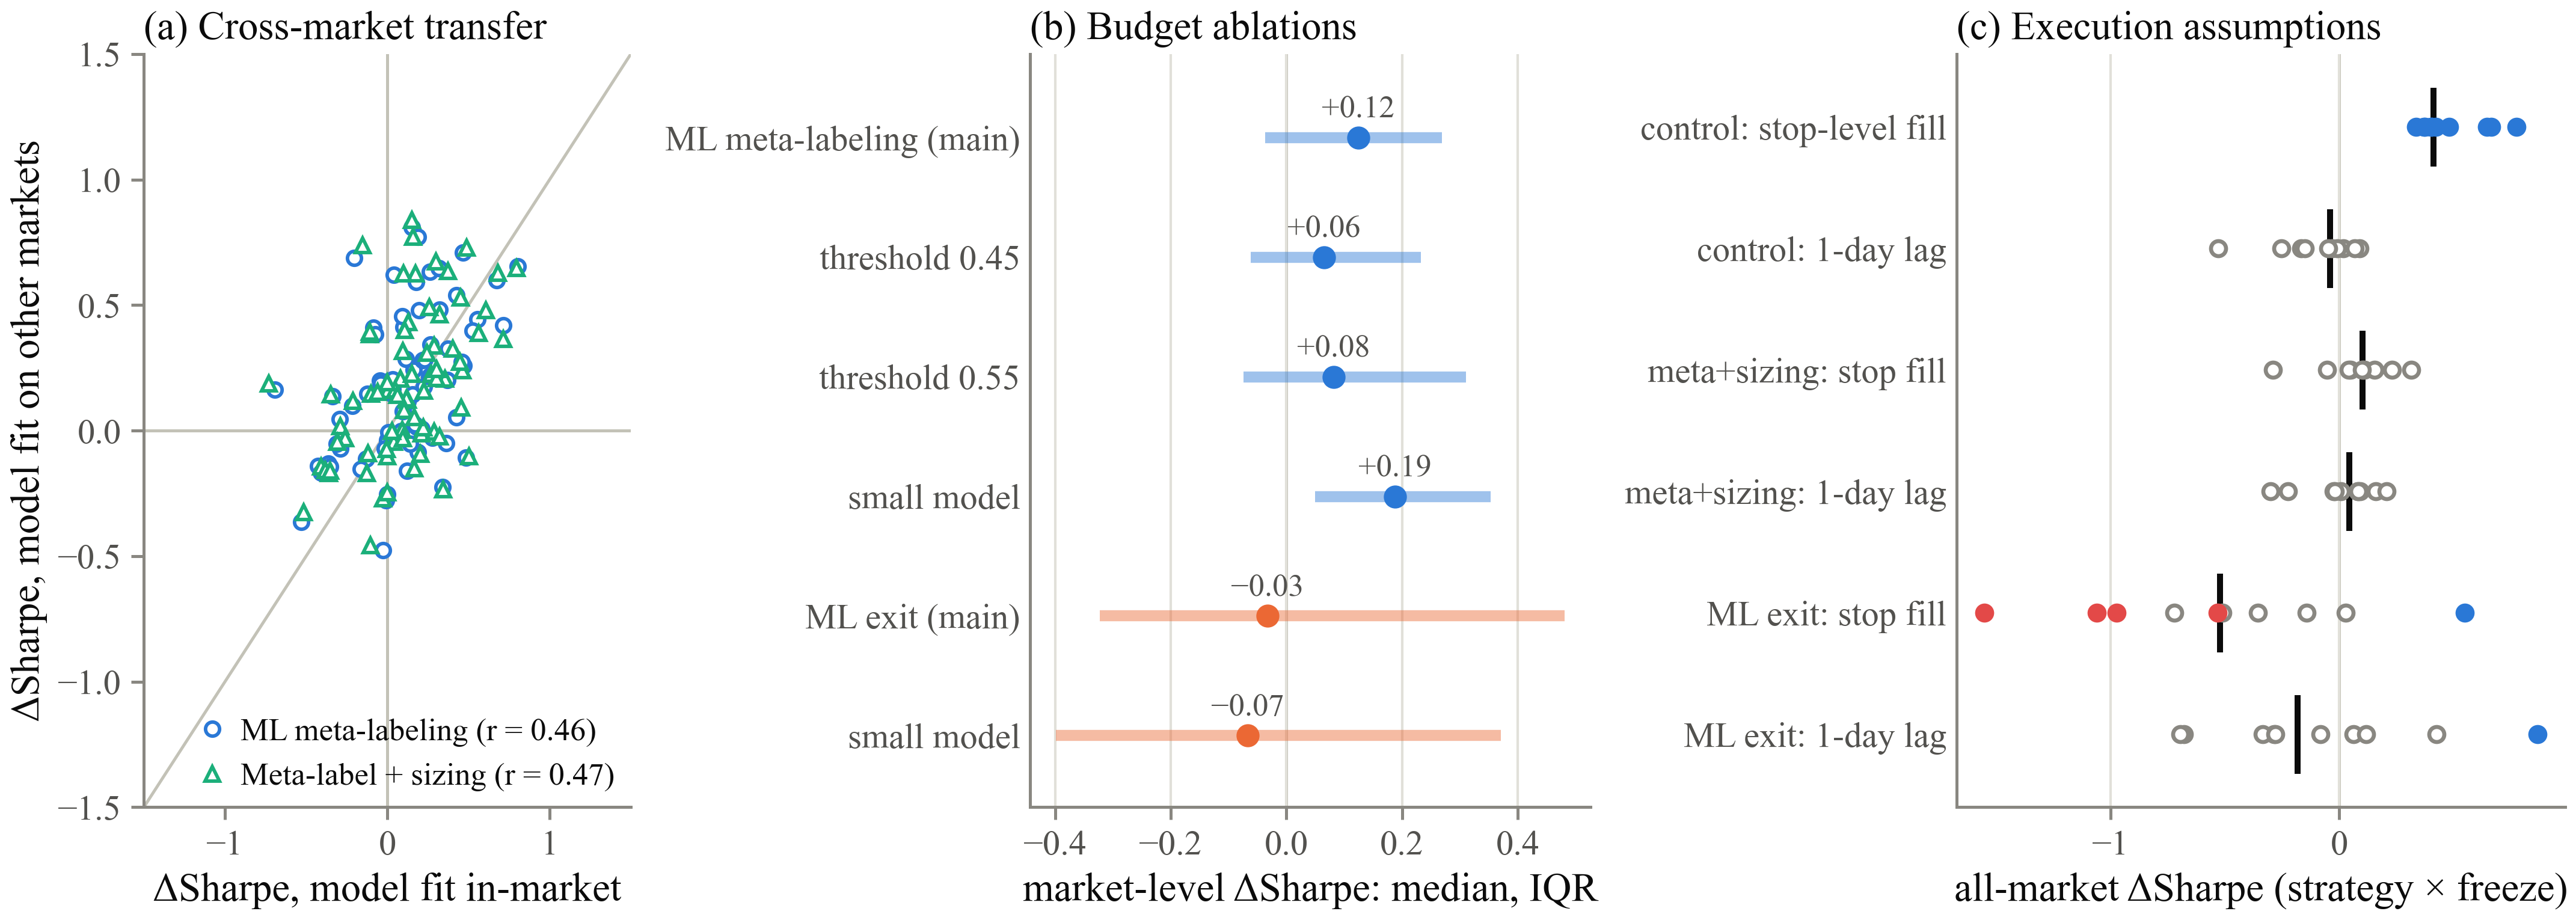
\includegraphics[width=7.14in]{figures/s2_robust.png}
\caption{Robustness. (a) Cross-market transfer: $\Delta$Sharpe of models fit on the other markets against models
fit in-market. (b) Budget ablations: median and interquartile range of market-level $\Delta$Sharpe. (c) Execution:
the control under stop-level fills or a one-day lag against the realistic control, and each ML variant against the
control under the same execution.}
\label{fig:s2robust}
\end{figure*}

\subsection{Transaction Costs}

The narrowing components are insensitive to transaction costs because they reduce turnover (Fig.~\ref{fig:s2costs}):
the median all-market $\Delta$Sharpe of meta-label + sizing is \STwoCostBestZero{}, \STwoCostBestOne{},
\STwoCostBestTwo{}, and \STwoCostBestFour{} at cost multipliers of zero, one, two, and four. ML exit, which raises
turnover, decays from \STwoCostExitZero{} to \STwoCostExitFour{} over the same range.

\begin{figure}[!t]
\centering
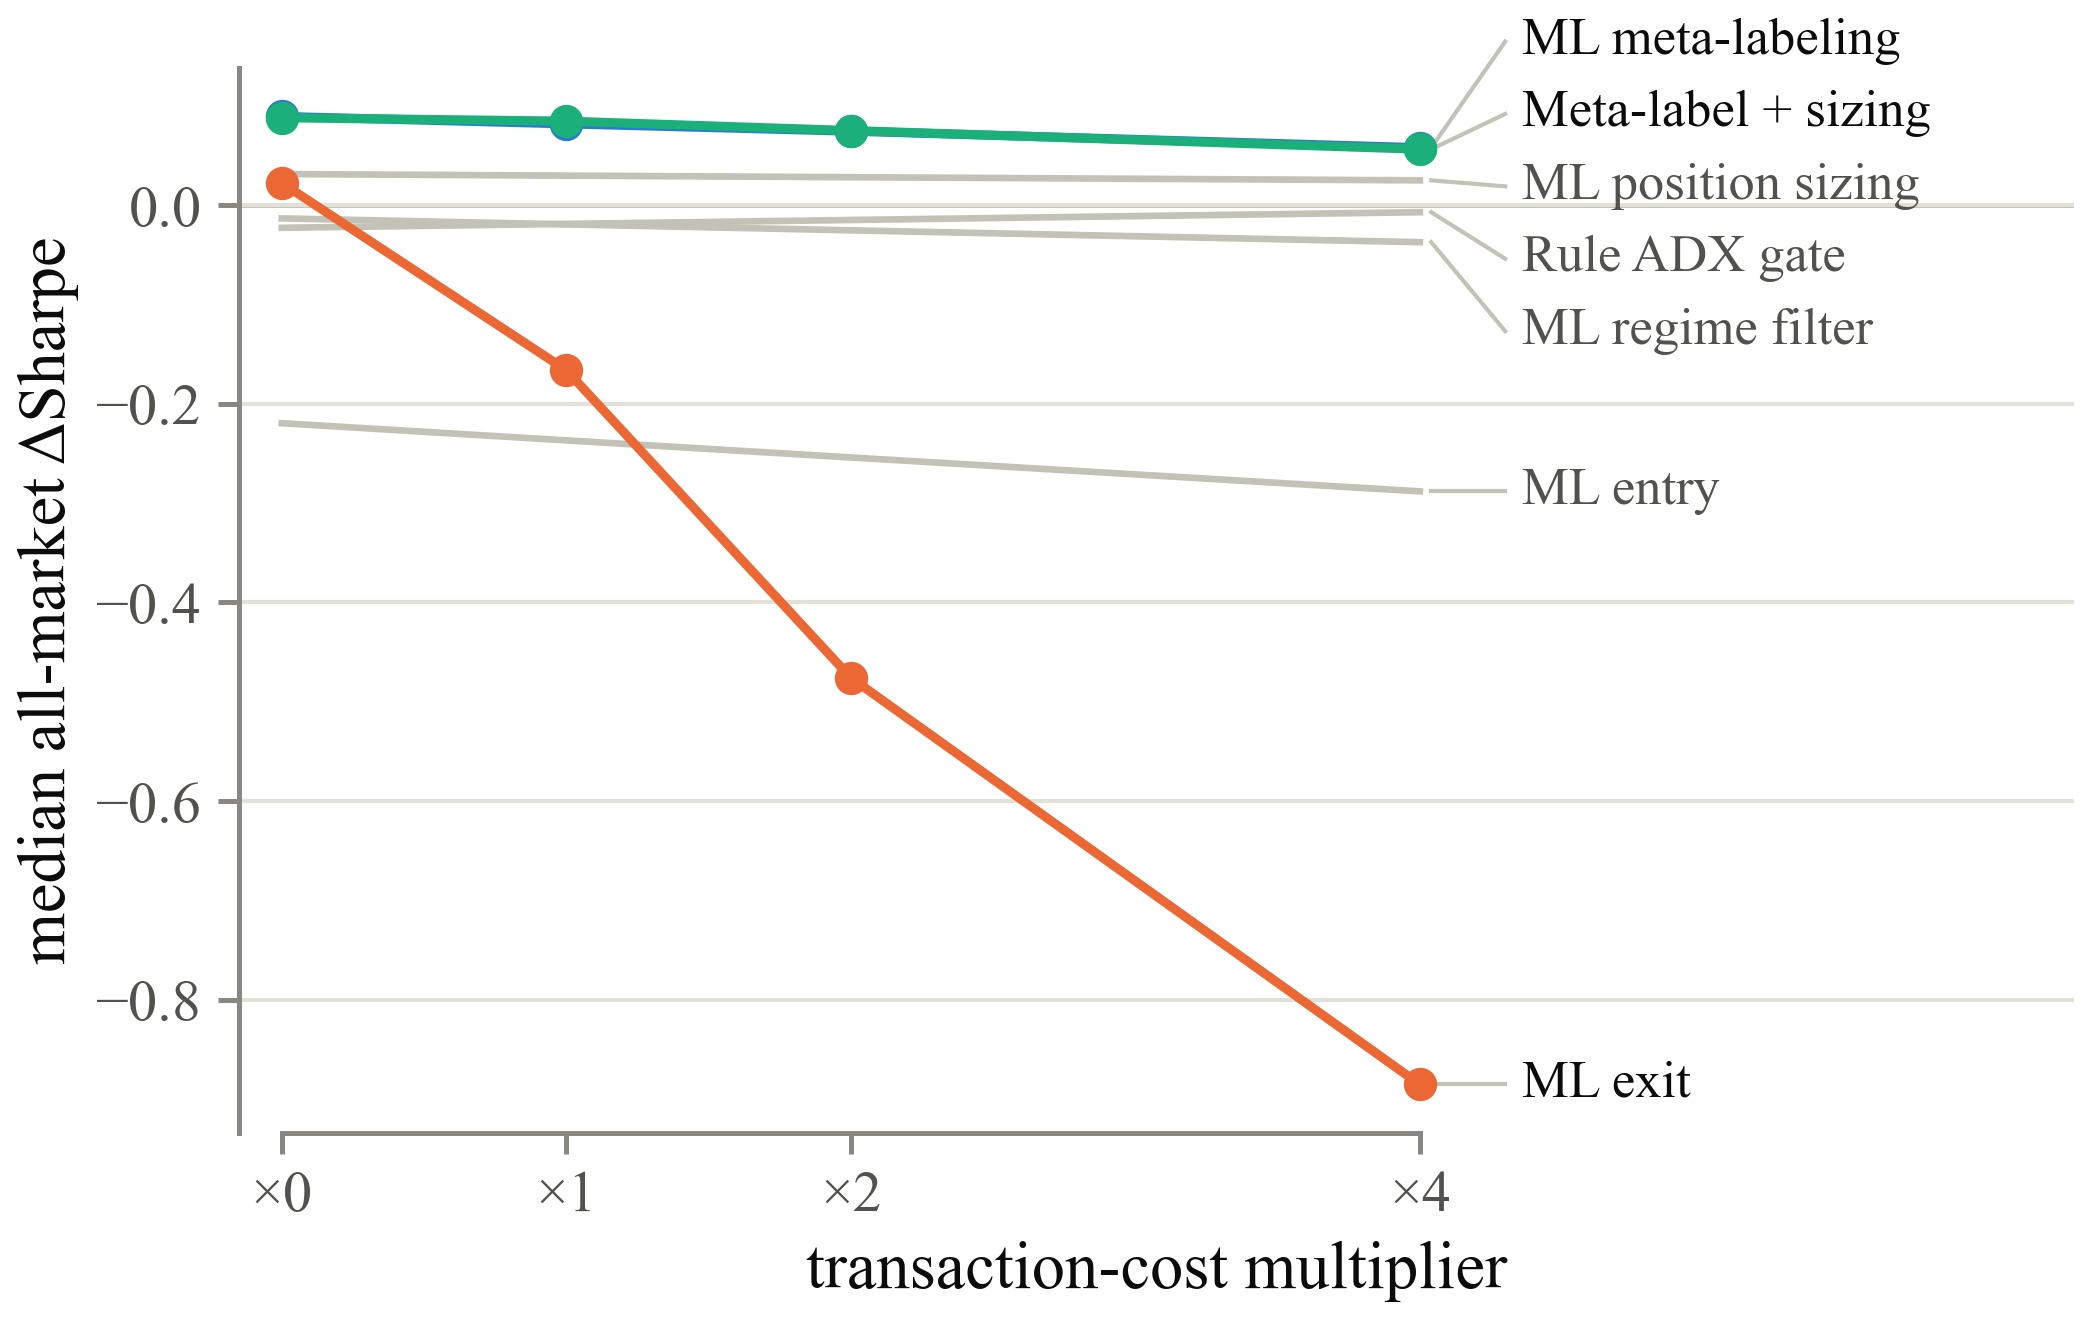
\includegraphics[width=3.487in]{figures/s2_costs.png}
\caption{Median all-market $\Delta$Sharpe by component as transaction costs are scaled. The meta-labeling and
meta-label + sizing lines nearly coincide.}
\label{fig:s2costs}
\end{figure}

\subsection{Regimes and Crises}

Narrowing components help in low-volatility regimes (meta-labeling \STwoRegMetaLowVol{}, meta-label + sizing
\STwoRegBestLowVol{}) and slightly hurt in high-volatility regimes (\STwoRegMetaHighVol{} and \STwoRegBestHighVol{});
ML exit helps in bear markets (\STwoRegExitBear{}) and hurts in bull markets (\STwoRegExitBull{}), consistent with
cutting trades early (Fig.~\ref{fig:regimes}a). The crisis windows show the exposure pattern of
Fig.~\ref{fig:s2risk} again: every component except ML entry makes the drawdown shallower in each of the five crises,
whereas ML entry, the only component that raises exposure, deepens it in each (Fig.~\ref{fig:regimes}c).

\begin{figure*}[!t]
\centering
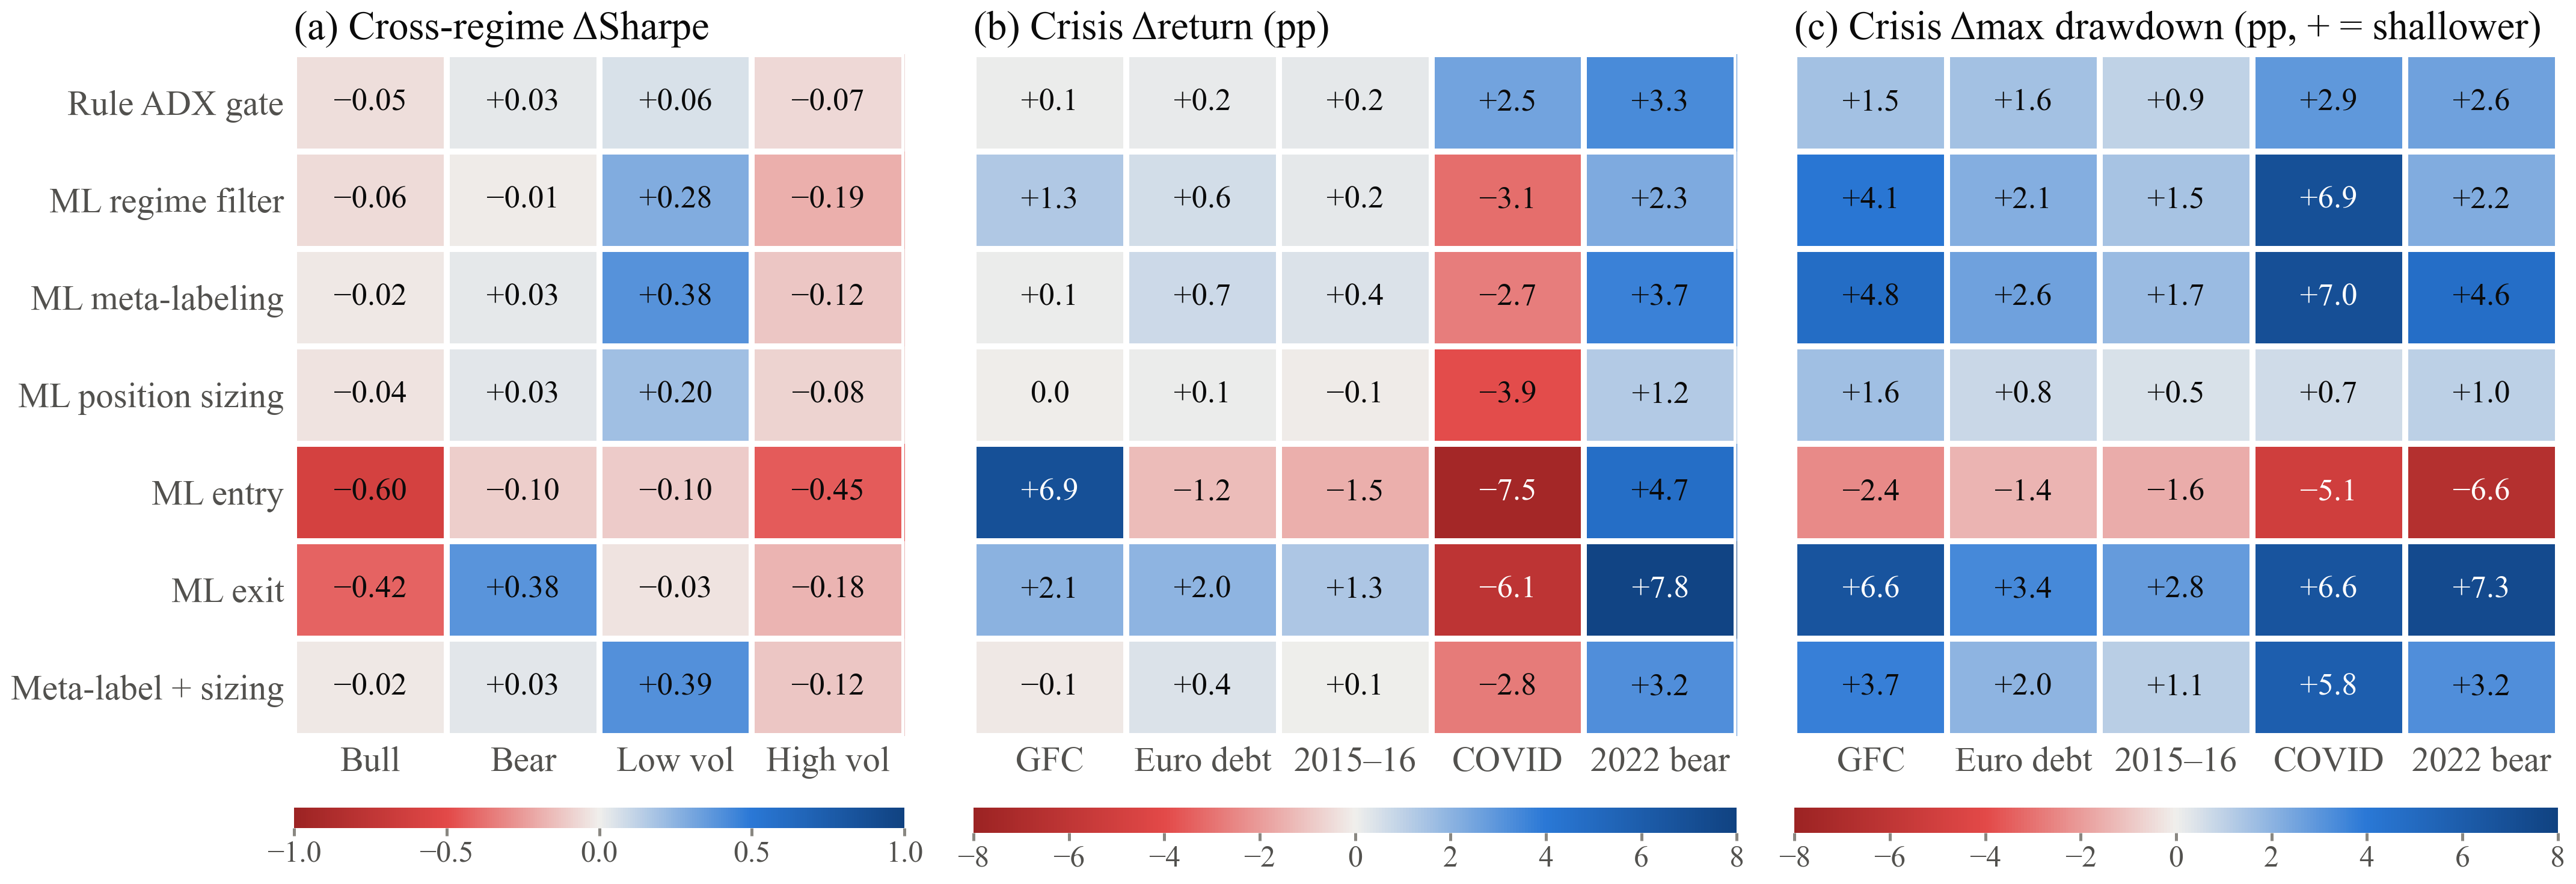
\includegraphics[width=7.14in]{figures/s2_regimes_crises.png}
\caption{Regimes and crises. (a) Mean all-market $\Delta$Sharpe within bull, bear, low-, and high-volatility regimes
defined from information at $t-1$. (b) Change in cumulative return and (c) change in maximum drawdown inside the five
pre-registered crisis windows, averaged over strategies (percentage points).}
\label{fig:regimes}
\end{figure*}

\subsection{Fragility and Parameter Decay}

Effects in survivorship-free markets and in current-constituent stocks and crypto are similar for the narrowing
components (meta-label + sizing median \STwoSurvBestFree{} vs.\ \STwoSurvBestProne{}; meta-labeling
\STwoSurvMetaFree{} vs.\ \STwoSurvMetaProne{}) and small for exit (\STwoSurvExitFree{} vs.\ \STwoSurvExitProne{}),
so survivorship does not drive the conclusions. Dropping any single instrument flips the sign of \STwoJackFlipShare{}
of market-level effects, so most of them are fragile, but none of the \STwoMktSigGain{}$+$\STwoMktSigLoss{} significant
ones (\STwoJackSigFlip{} flip; Fig.~\ref{fig:jackknife}); dropping any single market flips \STwoJackMarketFlipShare{}
of the global effects.

The controls' own parameter selection decays sharply out of sample (Fig.~\ref{fig:s2decay}). The dual SMA crossover
earns \STwoDecaySMAIs{} bps per trade in-sample and \STwoDecaySMAOos{} out-of-sample, and time-series momentum
\STwoDecayTSMOMIs{} and \STwoDecayTSMOMOos{}. The historical edge of these rules is largely absent since \STwoFzA{}
under realistic fills and costs, which bounds what any component can add.

\begin{figure}[!t]
\centering
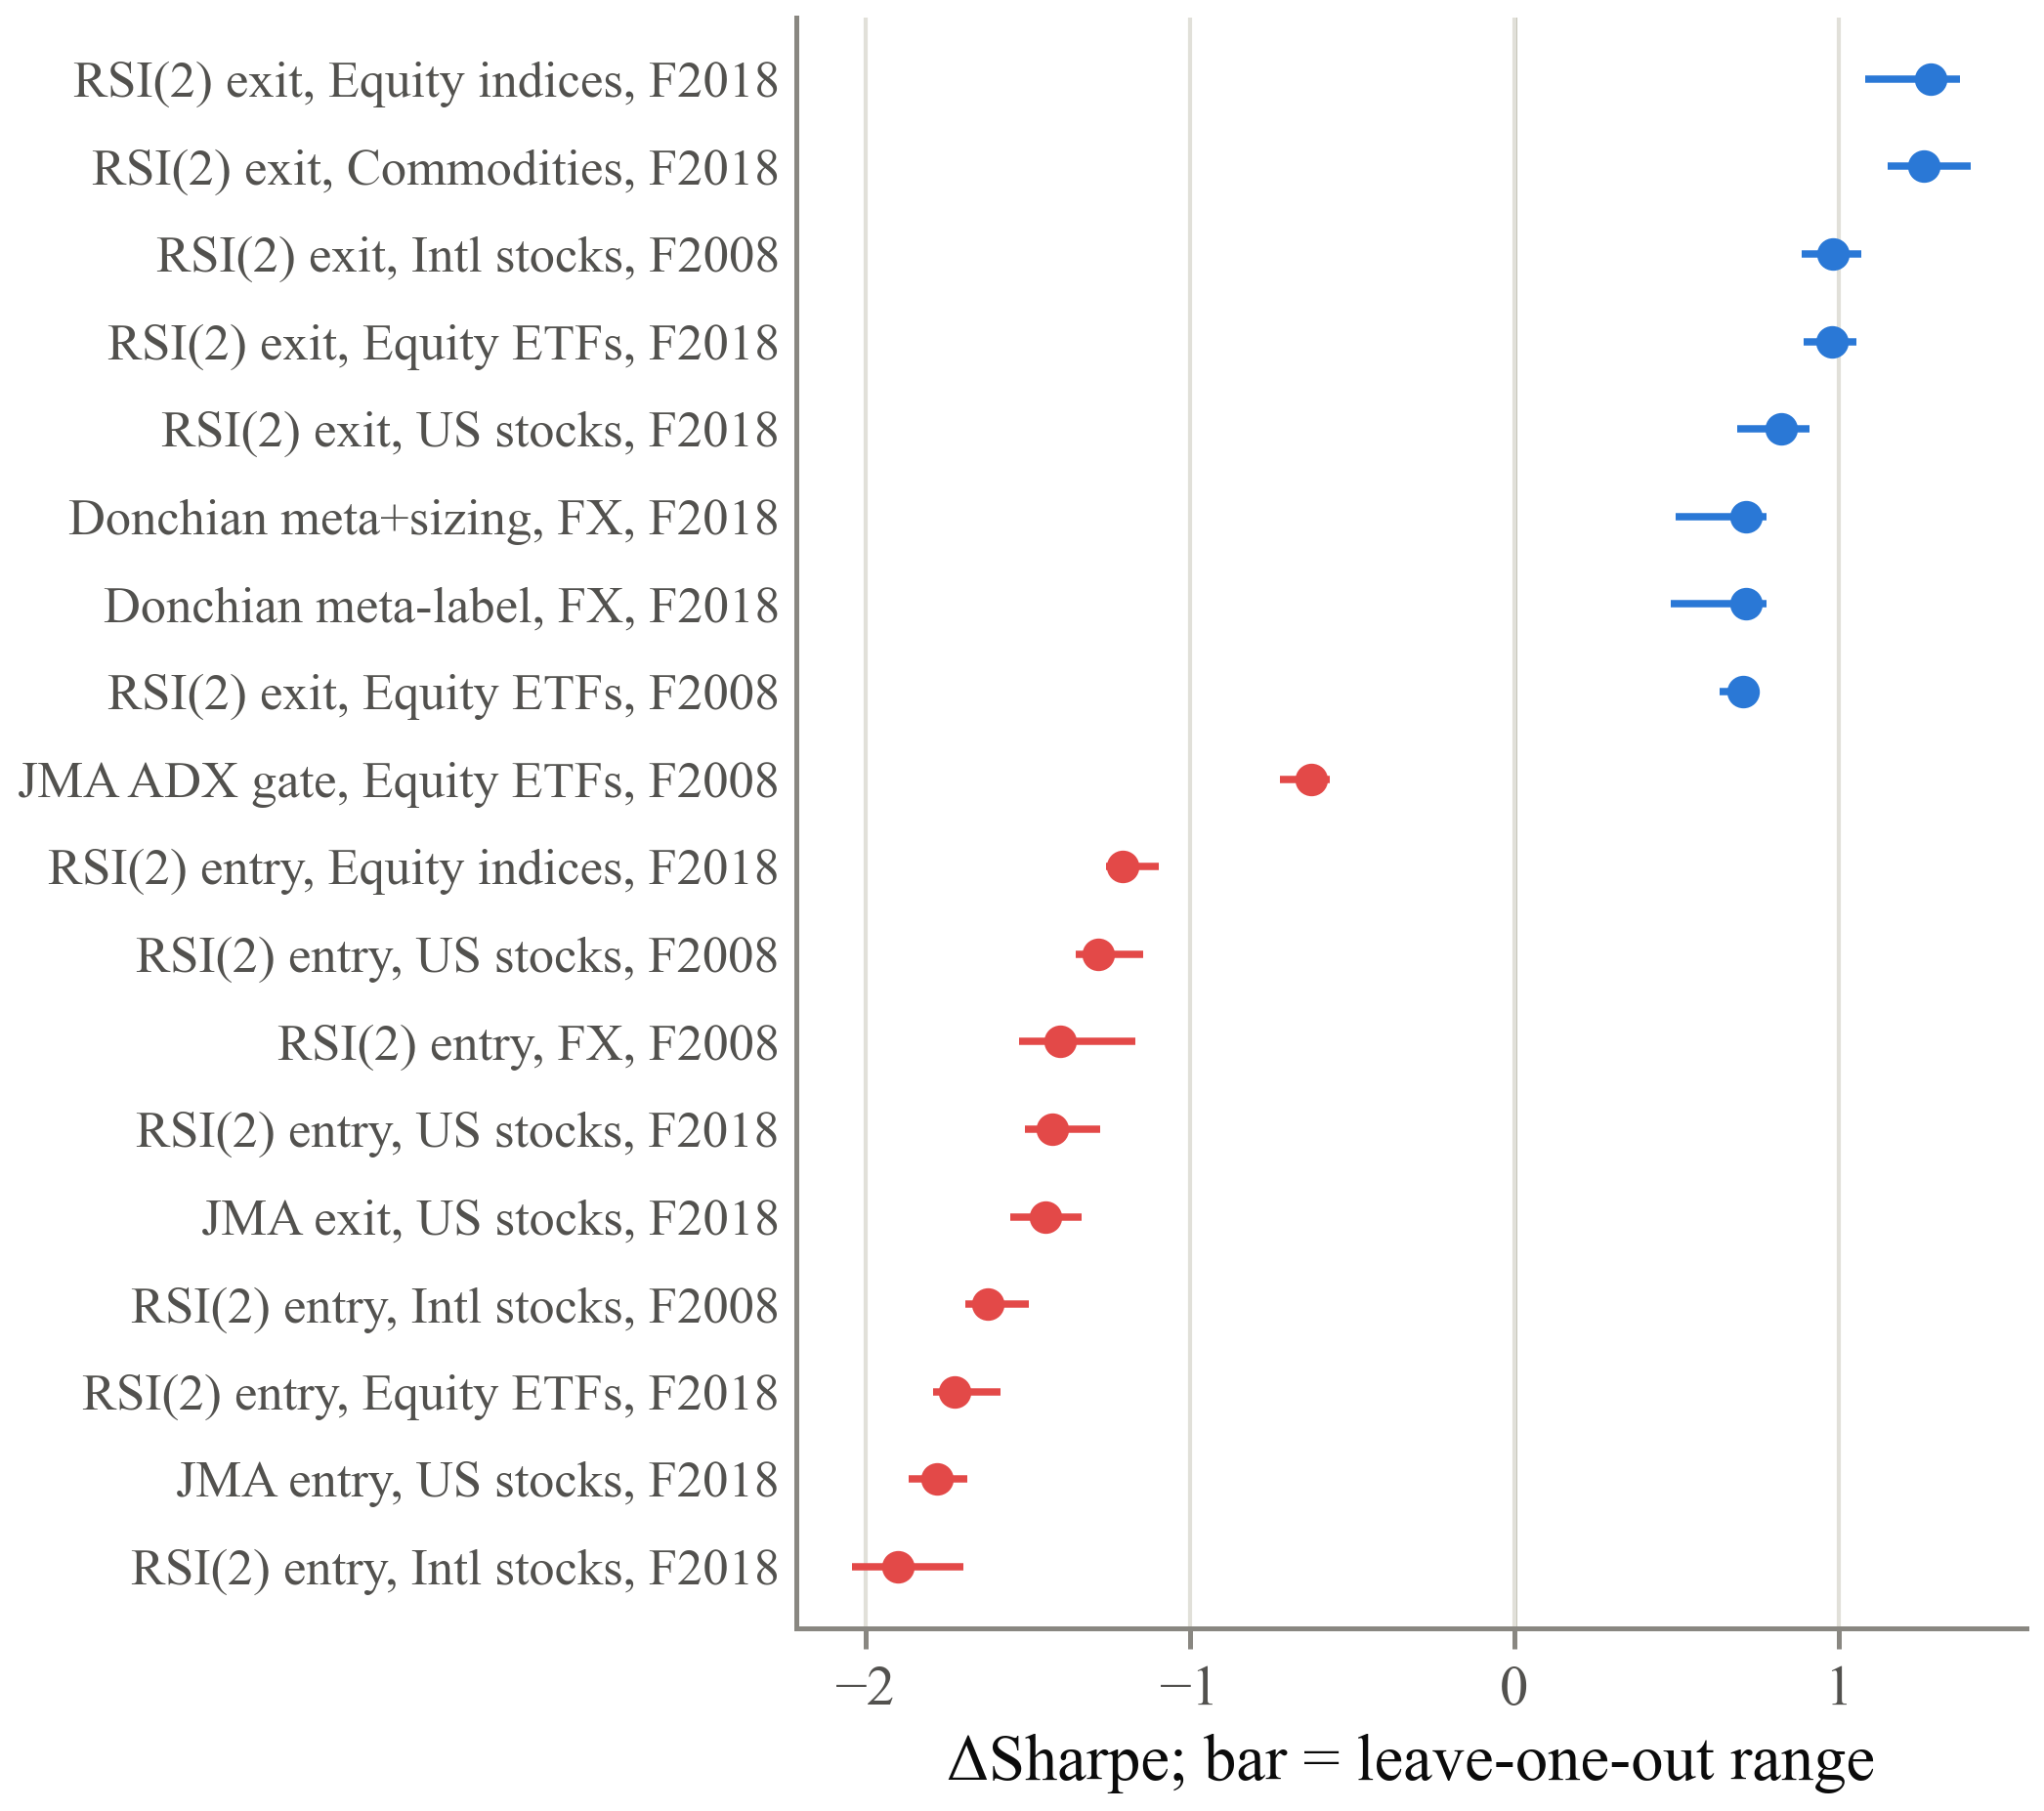
\includegraphics[width=3.487in]{figures/s2_jackknife.png}
\caption{Leave-one-instrument-out robustness of the \STwoMktSigGain{}$+$\STwoMktSigLoss{} significant market-level
effects: the full-sample $\Delta$Sharpe (dot) and its range when any one instrument is dropped (bar). No effect
changes sign.}
\label{fig:jackknife}
\end{figure}

\begin{figure}[!t]
\centering
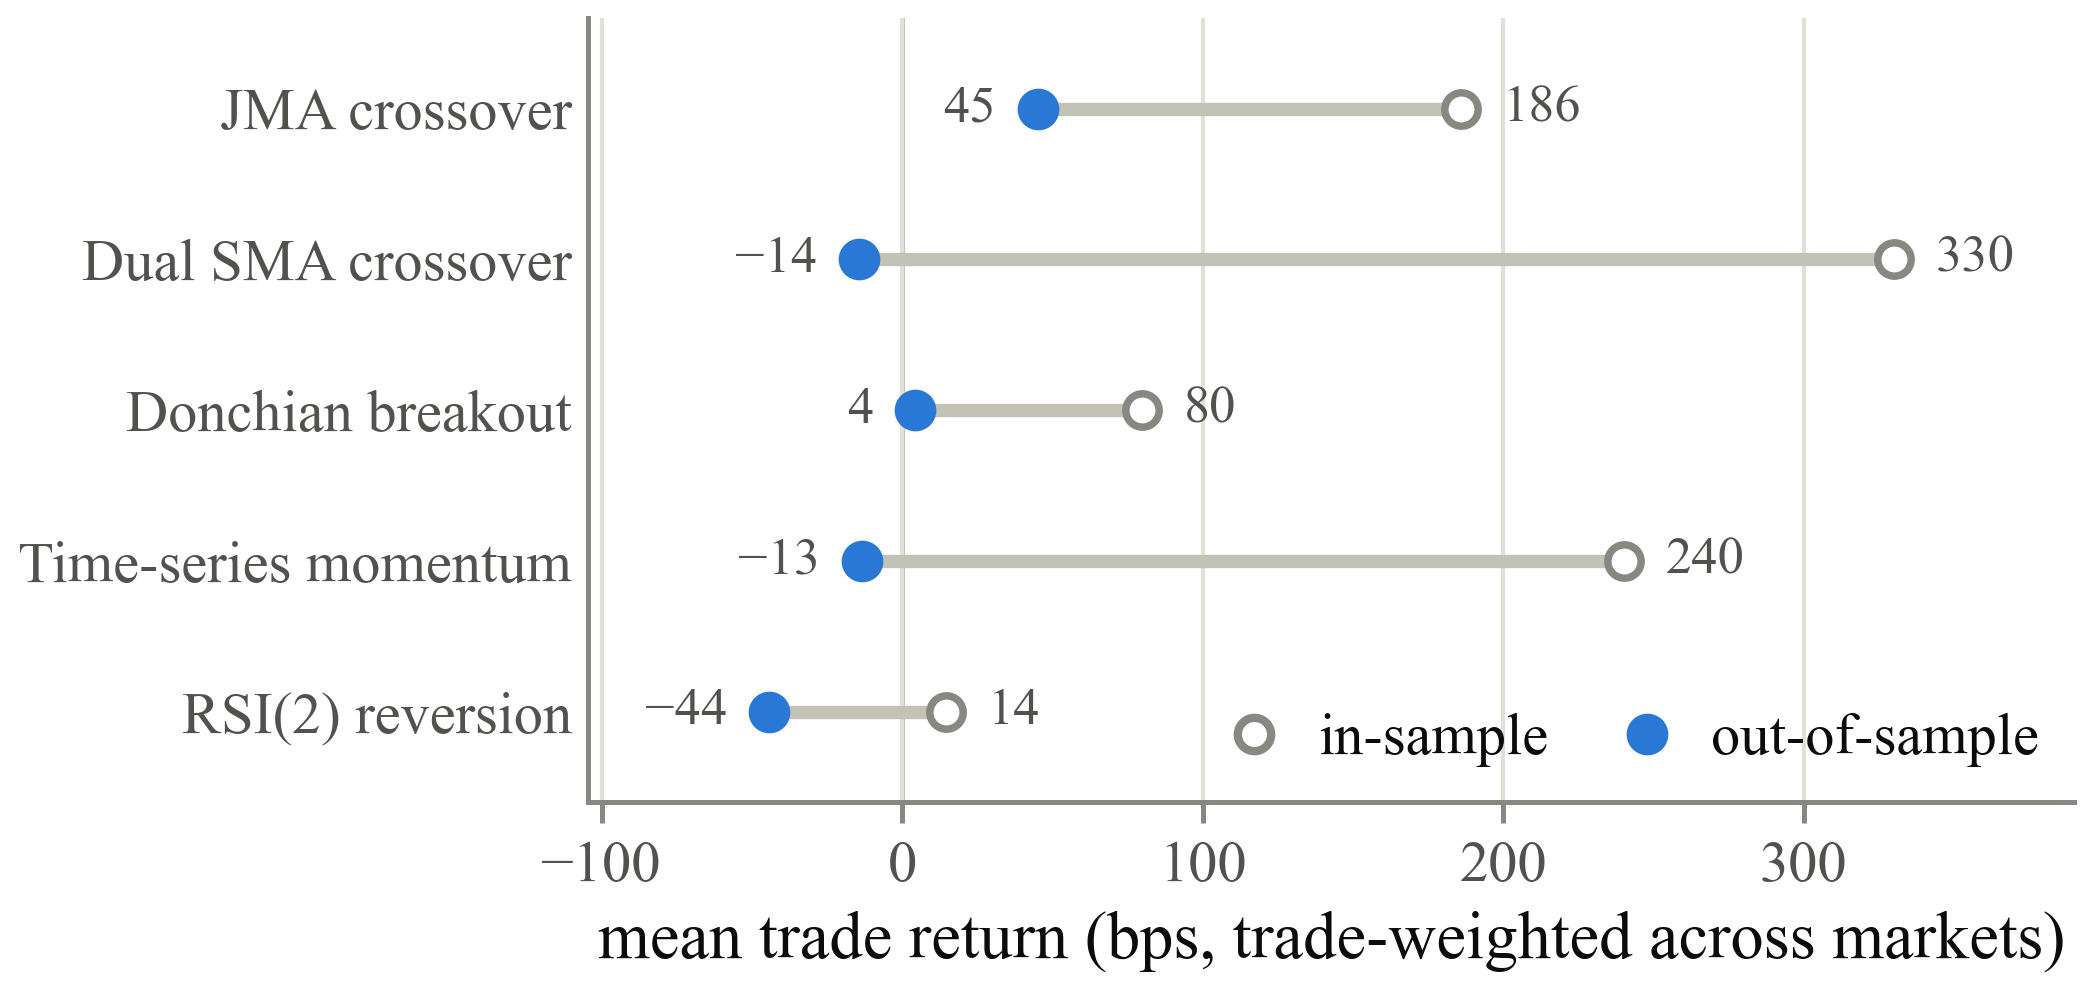
\includegraphics[width=3.487in]{figures/s2_decay.png}
\caption{Mean trade return of the walk-forward-selected controls in-sample and out-of-sample, trade-weighted across
markets.}
\label{fig:s2decay}
\end{figure}

\subsection{Bias Audit}

Table~\ref{tab:s2bias} lists each threat to validity named in the design, the test applied, and its outcome.

\begin{table*}[!t]
\centering
\caption{Bias audit: each threat to validity, the test applied, and its outcome.}
\label{tab:s2bias}
\footnotesize
\begin{tabular}{p{2.0cm} p{8.2cm} p{6.5cm}}
\toprule
Threat & Test applied & Outcome \\
\midrule
Look-ahead & Truncation invariance of every feature and every strategy signal (unit tests); regimes use $t-1$ data & pass (tests/test\_core.py, tests/test\_study2.py) \\
Data leakage & All models fit once before the freeze; scrambling all post-freeze data leaves every model bit-identical; labels straddling the freeze excluded & pass (tests) \\
Survivorship & Indices/ETFs/futures/FX analysed separately from current-constituent stocks and crypto & median $\Delta$SR meta-label+sizing: free \STwoSurvBestFree{} vs.\ prone \STwoSurvBestProne{} \\
Selection & Universe, strategies, components, windows, statistics pre-registered in git before data existed; every variant reported & study.toml first committed in 8d9f50f, before all data/results \\
Overfitting & Walk-forward parameter selection; deflated Sharpe; IS vs.\ OOS trade-return decay; two independent freezes & Fig.~\ref{fig:s2decay}; freeze agreement in Table~\ref{tab:s2comp} \\
Multiple testing & BH-FDR and Holm within families (528 market-level main tests) & raw $p<0.05$: \STwoMktRawSig{}; BH: \STwoMktSigGain{} gains / \STwoMktSigLoss{} losses; Holm: \STwoMktHolmSig{} \\
Execution realism & Close-fill of breached stops (default), 1-day entry lag, cost $\times$0--4, per-market costs & Fig.~\ref{fig:s2robust} \\
Data errors & Two independent sources (FRED) + browser spot-check (MarketWatch) & 5-day return corr.\ \STwoFredCorrFiveMin{}--\STwoFredCorrFiveMax{}; spot-check max diff \STwoSpotMaxDiff{} \\
\bottomrule
\end{tabular}
\end{table*}

